% Options for packages loaded elsewhere
\PassOptionsToPackage{unicode}{hyperref}
\PassOptionsToPackage{hyphens}{url}
\PassOptionsToPackage{dvipsnames,svgnames,x11names}{xcolor}
%
\documentclass[
  12pt,
  krantz2]{Format/krantzNoCorner}
\usepackage{amsmath,amssymb}
\usepackage{iftex}
\ifPDFTeX
  \usepackage[T1]{fontenc}
  \usepackage[utf8]{inputenc}
  \usepackage{textcomp} % provide euro and other symbols
\else % if luatex or xetex
  \usepackage{unicode-math} % this also loads fontspec
  \defaultfontfeatures{Scale=MatchLowercase}
  \defaultfontfeatures[\rmfamily]{Ligatures=TeX,Scale=1}
\fi
\usepackage{lmodern}
\ifPDFTeX\else
  % xetex/luatex font selection
\fi
% Use upquote if available, for straight quotes in verbatim environments
\IfFileExists{upquote.sty}{\usepackage{upquote}}{}
\IfFileExists{microtype.sty}{% use microtype if available
  \usepackage[]{microtype}
  \UseMicrotypeSet[protrusion]{basicmath} % disable protrusion for tt fonts
}{}
\makeatletter
\@ifundefined{KOMAClassName}{% if non-KOMA class
  \IfFileExists{parskip.sty}{%
    \usepackage{parskip}
  }{% else
    \setlength{\parindent}{0pt}
    \setlength{\parskip}{6pt plus 2pt minus 1pt}}
}{% if KOMA class
  \KOMAoptions{parskip=half}}
\makeatother
\usepackage{xcolor}
\usepackage{longtable,booktabs,array}
\usepackage{calc} % for calculating minipage widths
% Correct order of tables after \paragraph or \subparagraph
\usepackage{etoolbox}
\makeatletter
\patchcmd\longtable{\par}{\if@noskipsec\mbox{}\fi\par}{}{}
\makeatother
% Allow footnotes in longtable head/foot
\IfFileExists{footnotehyper.sty}{\usepackage{footnotehyper}}{\usepackage{footnote}}
\makesavenoteenv{longtable}
\usepackage{graphicx}
\makeatletter
\def\maxwidth{\ifdim\Gin@nat@width>\linewidth\linewidth\else\Gin@nat@width\fi}
\def\maxheight{\ifdim\Gin@nat@height>\textheight\textheight\else\Gin@nat@height\fi}
\makeatother
% Scale images if necessary, so that they will not overflow the page
% margins by default, and it is still possible to overwrite the defaults
% using explicit options in \includegraphics[width, height, ...]{}
\setkeys{Gin}{width=\maxwidth,height=\maxheight,keepaspectratio}
% Set default figure placement to htbp
\makeatletter
\def\fps@figure{htbp}
\makeatother
\setlength{\emergencystretch}{3em} % prevent overfull lines
\providecommand{\tightlist}{%
  \setlength{\itemsep}{0pt}\setlength{\parskip}{0pt}}
\setcounter{secnumdepth}{5}

\usepackage{booktabs}
\usepackage{empheq}
\setcounter{secnumdepth}{2}

\usepackage{amsfonts}
\usepackage{amsmath}
\usepackage{amssymb}
\usepackage{array}
\usepackage{caption}
\captionsetup[figureNoLabel]{labelformat=empty, justification=raggedright}

\usepackage{color}
\usepackage{colortbl}
\usepackage{xcolor}
\usepackage{xr}


\usepackage{fancyvrb}
\usepackage{framed}
\setlength{\fboxsep}{.8em}

\usepackage{graphicx}

\usepackage{multirow}
\usepackage{tabularx}

\usepackage{setspace}
\usepackage{scalefnt}

\usepackage{verbatim}
\usepackage{pdfpages}
\usepackage{mdframed}

\definecolor{lightgray}{gray}{0.98}

% Custom environment for background box
\newmdenv[
  backgroundcolor=lightgray,
  skipabove=10pt,
  skipbelow=10pt,
  leftmargin=0,
  rightmargin=0,
  innerleftmargin=10pt,
  innerrightmargin=10pt,
  innertopmargin=10pt,
  innerbottommargin=10pt
]{graybox}

\newenvironment{blackbox}{
  \definecolor{shadecolor}{rgb}{0, 0, 0}  % black
  \color{white}
  \begin{shaded}}
 {\end{shaded}}
 
% \newenvironment{greybox}{
%   \definecolor{shadecolor}{rgb}{0.9, 0.9, 0.9}  % light grey??
%   \color{white}
%   \begin{shaded}}
%  {\end{shaded}}
 
% \usepackage[left=1in,top=1in,right=1in,bottom=1in]{geometry}



%\usepackage{wrapfig}



\setlength{\fboxsep}{.8em}

\renewcommand{\hrulefill}{%
  \leavevmode\leaders\hrule height 2pt\hfill\kern0pt }
  
\renewcommand{\dotfill}{%
  \leavevmode\cleaders\hbox to 0.60em{\hss .\hss }\hfill\kern0pt }
  


\usepackage{makeidx}
\makeindex

\usepackage{booktabs}
\usepackage{longtable}
\usepackage{array}
\usepackage{multirow}
\usepackage{wrapfig}
\usepackage{float}
\usepackage{colortbl}
\usepackage{pdflscape}
\usepackage{tabu}
\usepackage{threeparttable}
\usepackage{threeparttablex}
\usepackage[normalem]{ulem}
\usepackage{makecell}
\usepackage{xcolor}
\ifLuaTeX
  \usepackage{selnolig}  % disable illegal ligatures
\fi
\usepackage[]{natbib}
\bibliographystyle{Format/econPeriod}
\IfFileExists{bookmark.sty}{\usepackage{bookmark}}{\usepackage{hyperref}}
\IfFileExists{xurl.sty}{\usepackage{xurl}}{} % add URL line breaks if available
\urlstyle{same}
\hypersetup{
  colorlinks=true,
  linkcolor={Maroon},
  filecolor={Maroon},
  citecolor={Blue},
  urlcolor={Blue},
  pdfcreator={LaTeX via pandoc}}

\author{}
\date{\vspace{-2.5em}}

\begin{document}


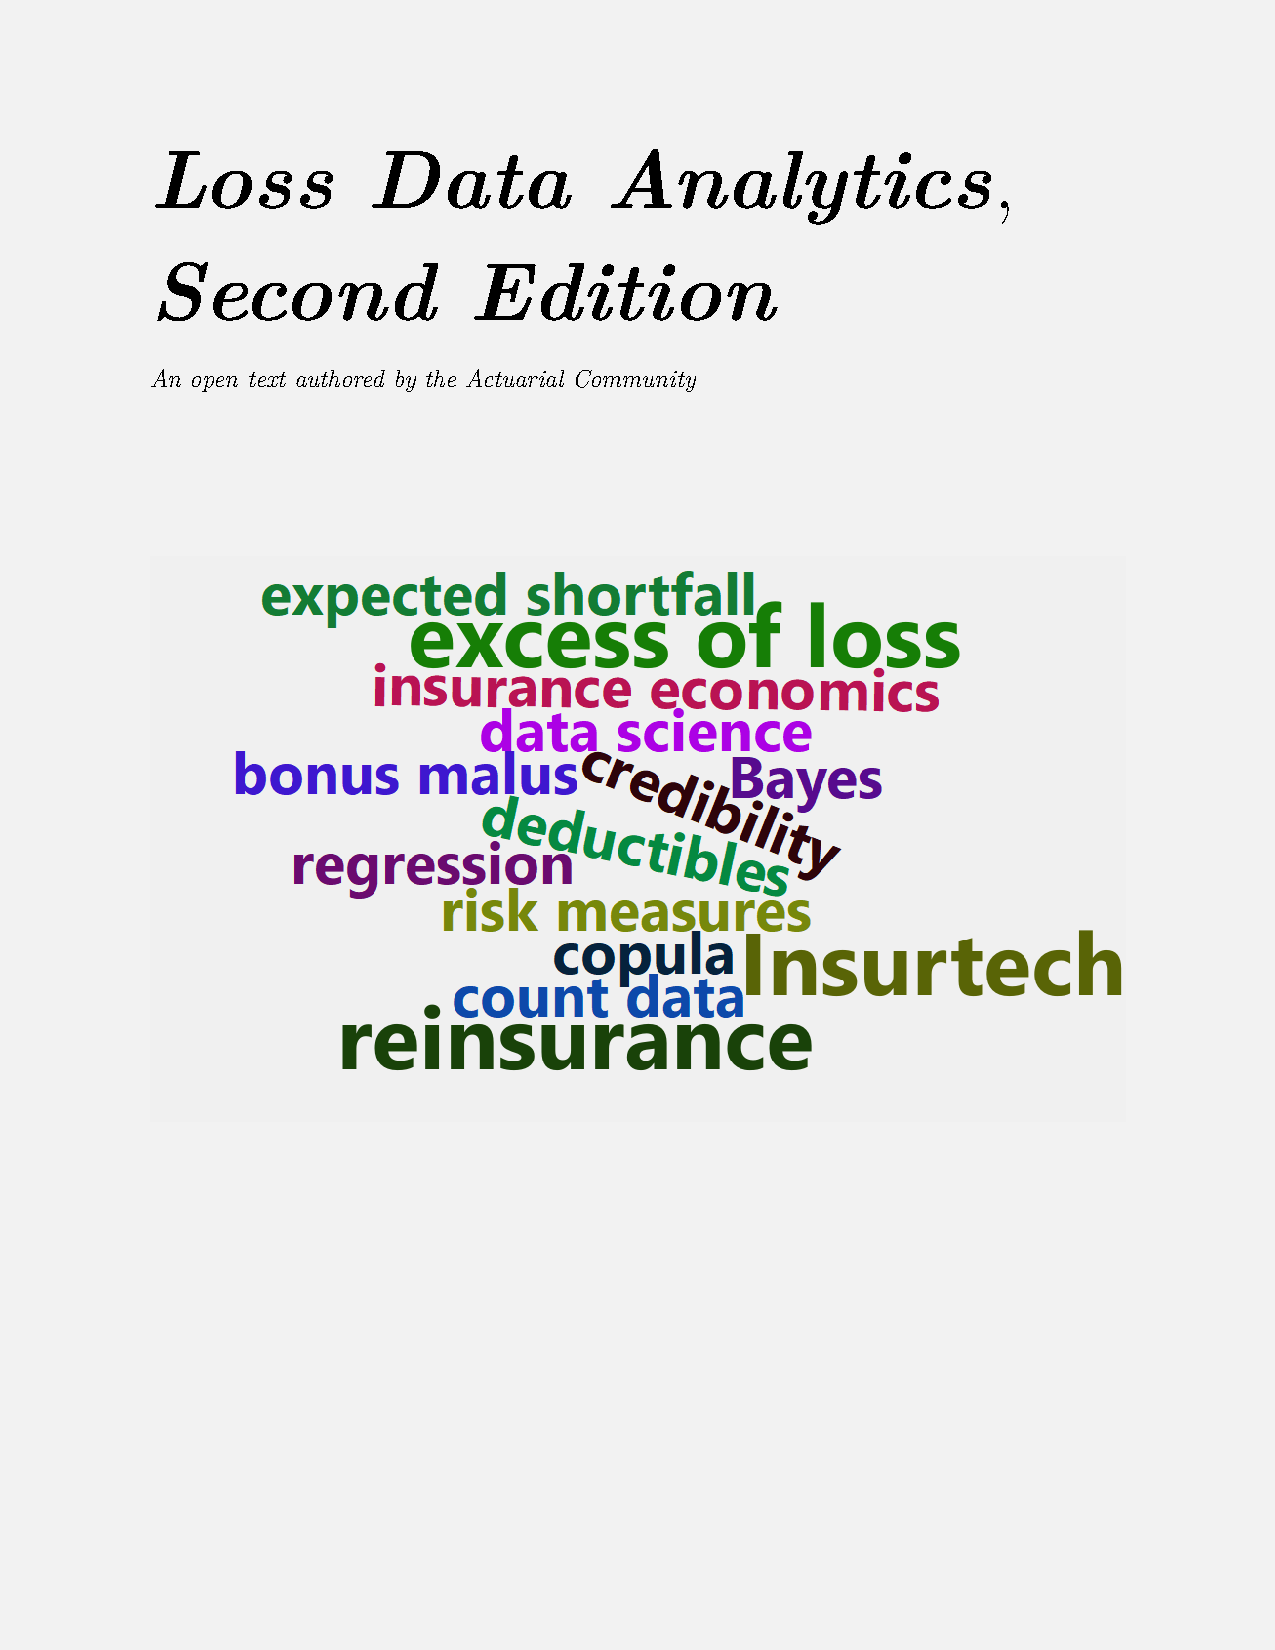
\includepdf[fitpaper=true, scale = 1.1]{"Figures/FreesCoverIdea19Sept2024.pdf"}  

{
\hypersetup{linkcolor=}
\setcounter{tocdepth}{2}
\tableofcontents
}
\hypertarget{preface}{%
\chapter*{Preface}\label{preface}}


\emph{Date: 19 September 2024}

\hypertarget{book-description}{%
\subsubsection*{Book Description}\label{book-description}}


\textbf{Loss Data Analytics} is an interactive, online, freely available text.

\begin{itemize}
\tightlist
\item
  The online version contains many interactive objects (quizzes, computer demonstrations, interactive graphs, video, and the like) to promote \emph{deeper learning}.
\item
  A subset of the book is available for \emph{offline reading} in pdf and EPUB formats.
\item
  The online text will be available in multiple languages to promote access to a \emph{worldwide audience}.
\end{itemize}

\hypertarget{what-will-success-look-like}{%
\subsubsection*{What will success look like?}\label{what-will-success-look-like}}


The online text will be freely available to a worldwide audience. The online version will contain many interactive objects (quizzes, computer demonstrations, interactive graphs, video, and the like) to promote deeper learning. Moreover, a subset of the book will be available in pdf format for low-cost printing. The online text will be available in multiple languages to promote access to a worldwide audience.

\hypertarget{how-will-the-text-be-used}{%
\subsubsection*{How will the text be used?}\label{how-will-the-text-be-used}}


This book will be useful in actuarial curricula worldwide. It will cover the loss data learning objectives of the major actuarial organizations. Thus, it will be suitable for classroom use at universities as well as for use by independent learners seeking to pass professional actuarial examinations. Moreover, the text will also be useful for the continuing professional development of actuaries and other professionals in insurance and related financial risk management industries.

\hypertarget{why-is-this-good-for-the-profession}{%
\subsubsection*{Why is this good for the profession?}\label{why-is-this-good-for-the-profession}}


An online text is a type of open educational resource (OER). One important benefit of an OER is that it equalizes access to knowledge, thus permitting a broader community to learn about the actuarial profession. Moreover, it has the capacity to engage viewers through active learning that deepens the learning process, producing analysts more capable of solid actuarial work.

Why is this good for students and teachers and others involved in the learning process? Cost is often cited as an important factor for students and teachers in textbook selection (see a recent post on the \href{https://www.aei.org/publication/the-new-era-of-the-400-college-textbook-which-is-part-of-the-unsustainable-higher-education-bubble/}{\$400 textbook}). Students will also appreciate the ability to ``carry the book around'' on their mobile devices.

\hypertarget{why-loss-data-analytics}{%
\subsubsection*{Why loss data analytics?}\label{why-loss-data-analytics}}


The intent is that this type of resource will eventually permeate throughout the actuarial curriculum. Given the dramatic changes in the way that actuaries treat data, loss data seems like a natural place to start. The idea behind the name \emph{loss data analytics} is to integrate classical loss data models from applied probability with modern analytic tools. In particular, we recognize that big data (including social media and usage based insurance) are here to stay and that high speed computation is readily available.

\hypertarget{project-goal}{%
\subsubsection*{Project Goal}\label{project-goal}}


The project goal is to have the actuarial community author our textbooks in a collaborative fashion. To get involved, please visit our
\href{https://sites.google.com/a/wisc.edu/loss-data-analytics/}{Open Actuarial Textbooks Project Site}.

\hypertarget{acknowledgements}{%
\section*{Acknowledgements}\label{acknowledgements}}


Edward Frees acknowledges the John and Anne Oros Distinguished Chair for Inspired Learning in Business which provided seed money to support the project. Frees and his Wisconsin colleagues also acknowledge a Society of Actuaries Center of Excellence Grant that provided funding to support work in dependence modeling and health initiatives. Wisconsin also provided an education innovation grant that provided partial support for the many students who have worked on this project.

We acknowledge the Society of Actuaries for permission to use problems from their examinations.

We thank Rob Hyndman, Monash University, for allowing us to use his excellent style files to produce the online version of the book.

We thank Yihui Xie and his colleagues at \href{https://www.rstudio.com/}{Rstudio} for the \href{https://bookdown.org/yihui/bookdown/}{R bookdown} package that allows us to produce this book.

We also wish to acknowledge the support and sponsorship of the \href{http://www.blackactuaries.org/}{International Association of Black Actuaries} in our joint efforts to provide actuarial educational content to all.


\includegraphics[width=0.25\textwidth,height=\textheight]{Figures/IABA.png}

\hypertarget{contributors}{%
\section*{Contributors}\label{contributors}}


The project goal is to have the actuarial community author our textbooks in a collaborative fashion. The following contributors have taken a leadership role in developing \emph{Loss Data Analytics}.

\begin{center}\rule{0.5\linewidth}{0.5pt}\end{center}

\begin{center}
\includegraphics[width=0.2\linewidth,height=0.3\textheight]{ContributorPics/ZeinabAmin} \end{center}

\begin{center}
\textbf{ Zeinab Amin }
\end{center}

\begin{itemize}
\item
  \textbf{Zeinab Amin} is a Professor at the Department of Mathematics and Actuarial Science and Associate Provost for Assessment and Accreditation at the American University in Cairo (AUC). Amin holds a PhD in Statistics and is an Associate of the Society of Actuaries. Amin is the recipient of the 2016 Excellence in Academic Service Award and the 2009 Excellence in Teaching Award from AUC. Amin has designed and taught a variety of statistics and actuarial science courses. Amin's current area of research includes quantitative risk assessment, reliability assessment, general statistical modelling, and Bayesian statistics.
\item
  \textbf{Katrien Antonio}, KU Leuven
\end{itemize}

\begin{center}\rule{0.5\linewidth}{0.5pt}\end{center}

\newpage

\begin{center}
\includegraphics[width=0.2\linewidth,height=0.3\textheight]{ContributorPics/JFBegin} \end{center}

\begin{center}
\textbf{ Jean-François Bégin }
\end{center}

\begin{itemize}
\item
  \textbf{Jean-François Bégin} is an Assistant Professor in the Department of Statistics and Actuarial Science at Simon Fraser University in British Columbia, Canada. Bégin holds a PhD in Financial Engineering from HEC Montréal, Canada, and is a Fellow of the Society of Actuaries and of the Canadian Institute of Actuaries. His current research interests include financial modelling, financial econometrics, Bayesian statistics, filtering methods, credit risk, option pricing, and pension economics. Bégin has designed and taught a variety of actuarial finance and actuarial communication courses.
\item
  \textbf{Jan Beirlant}, KU Leuven
\end{itemize}

\begin{center}\rule{0.5\linewidth}{0.5pt}\end{center}

\begin{center}
\includegraphics[width=0.2\linewidth,height=0.3\textheight]{ContributorPics/Charpentier} \end{center}

\begin{center}
\textbf{ Arthur Charpentier }
\end{center}

\begin{itemize}
\tightlist
\item
  \textbf{Arthur Charpentier} is a professor in the Department of Mathematics at the Université du Québec á Montréal.~Prior to that, he worked at a large general insurance company in Hong Kong, China, and the French Federation of Insurers in Paris, France. He received a MS on mathematical economics at Université Paris Dauphine and a MS in actuarial science at ENSAE (National School of Statistics) in Paris, and a PhD degree from KU Leuven, Belgium. His research interests include econometrics, applied probability and actuarial science. He has published several books (the most recent one on \emph{Computational Actuarial Science with R}, CRC) and papers on a variety of topics. He is a Fellow of the French Institute of Actuaries, and was in charge of the `Data Science for Actuaries' program from 2015 to 2018.
\end{itemize}

\begin{center}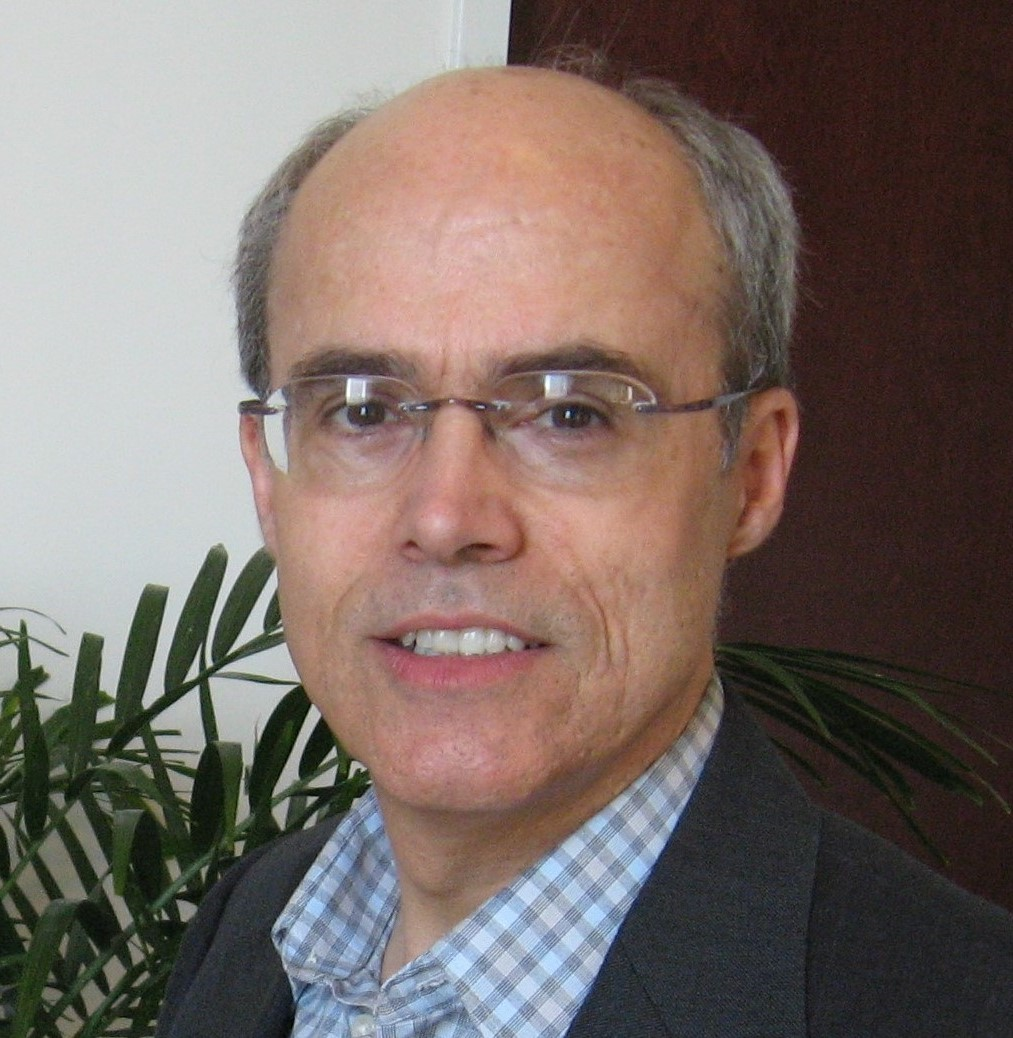
\includegraphics[width=0.2\linewidth,height=0.3\textheight]{ContributorPics/PhotoGaryDean} \end{center}

\begin{center}
\textbf{ Curtis Gary Dean }
\end{center}

\begin{itemize}
\tightlist
\item
  \textbf{Curtis Gary Dean} is the Lincoln Financial Distinguished Professor of Actuarial Science at Ball State University. He is a Fellow of the Casualty Actuarial Society and a CFA charterholder. He has extensive practical experience as an actuary at American States Insurance, SAFECO, and Travelers. He has served the CAS and actuarial profession as chair of the Examination Committee, first editor-in-chief for \emph{Variance: Advancing the Science of Risk}, and as a member of the Board of Directors and the Executive Council. He contributed a chapter to \emph{Predictive Modeling Applications in Actuarial Science} published by Cambridge University Press.
\end{itemize}

\begin{center}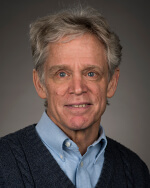
\includegraphics[width=0.2\linewidth,height=0.3\textheight]{ContributorPics/Frees_Jed2018_150x188} \end{center}

\begin{center}
\textbf{ Edward (Jed) Frees }
\end{center}

\begin{itemize}
\tightlist
\item
  \textbf{Edward (Jed) Frees} is an emeritus professor, formerly the Hickman-Larson Chair of Actuarial Science at the University of Wisconsin-Madison. He is a Fellow of both the Society of Actuaries and the American Statistical Association. He has published extensively (a four-time winner of the Halmstad and Prize for best paper published in the actuarial literature) and has written three books. He also is a co-editor of the two-volume series \emph{Predictive Modeling Applications in Actuarial Science} published by Cambridge University Press.
\end{itemize}

\newpage

\begin{center}
\includegraphics[width=0.2\linewidth,height=0.3\textheight]{ContributorPics/GuojunGan} \end{center}

\begin{center}
\textbf{ Guojun Gan }
\end{center}

\begin{itemize}
\tightlist
\item
  \textbf{Guojun Gan} is an associate professor in the Department of Mathematics at the University of Connecticut, where he has been since August 2014. Prior to that, he worked at a large life insurance company in Toronto, Canada for six years. He received a BS degree from Jilin University, Changchun, China, in 2001 and MS and PhD degrees from York University, Toronto, Canada, in 2003 and 2007, respectively. His research interests include data mining and actuarial science. He has published several books and papers on a variety of topics, including data clustering, variable annuity, mathematical finance, applied statistics, and VBA programming.
\end{itemize}

\begin{center}
\includegraphics[width=0.2\linewidth,height=0.3\textheight]{ContributorPics/Gao_Lisa_150x188} \end{center}

\begin{center}
\textbf{ Lisa Gao }
\end{center}

\begin{itemize}
\tightlist
\item
  \textbf{Lisa Gao} is a PhD candidate in the Risk and Insurance department at the University of Wisconsin-Madison. She holds a BMath in Actuarial Science and Statistics from the University of Waterloo and is an Associate of the Society of Actuaries.
\end{itemize}

\begin{itemize}
\tightlist
\item
  \textbf{José Garrido}, Concordia University
\end{itemize}

\begin{center}\rule{0.5\linewidth}{0.5pt}\end{center}

\begin{center}
\includegraphics[width=0.2\linewidth,height=0.3\textheight]{ContributorPics/Larry2018} \end{center}

\begin{center}
\textbf{ Lei (Larry) Hua }
\end{center}

\begin{itemize}
\tightlist
\item
  \textbf{Lei (Larry) Hua} is an Associate Professor of Actuarial Science at Northern Illinois University. He earned a PhD degree in Statistics from the University of British Columbia. He is an Associate of the Society of Actuaries. His research work focuses on multivariate dependence modeling for non-Gaussian phenomena and innovative applications for financial and insurance industries.
\end{itemize}

\begin{center}
\includegraphics[width=0.2\linewidth,height=0.3\textheight]{ContributorPics/Noriszura} \end{center}

\begin{center}
\textbf{ Noriszura Ismail }
\end{center}

\begin{itemize}
\tightlist
\item
  \textbf{Noriszura Ismail} is a Professor and Head of Actuarial Science Program, Universiti Kebangsaan Malaysia (UKM). She specializes in Risk Modelling and Applied Statistics. She obtained her BSc and MSc (Actuarial Science) in 1991 and 1993 from University of Iowa, and her PhD (Statistics) in 2007 from UKM. She also passed several papers from Society of Actuaries in 1994. She has received several research grants from Ministry of Higher Education Malaysia (MOHE) and UKM, totaling about MYR1.8 million. She has successfully supervised and co-supervised several PhD students (13 completed and 11 on-going). She currently has about 180 publications, consisting of 88 journals and 95 proceedings.
\end{itemize}

\begin{center}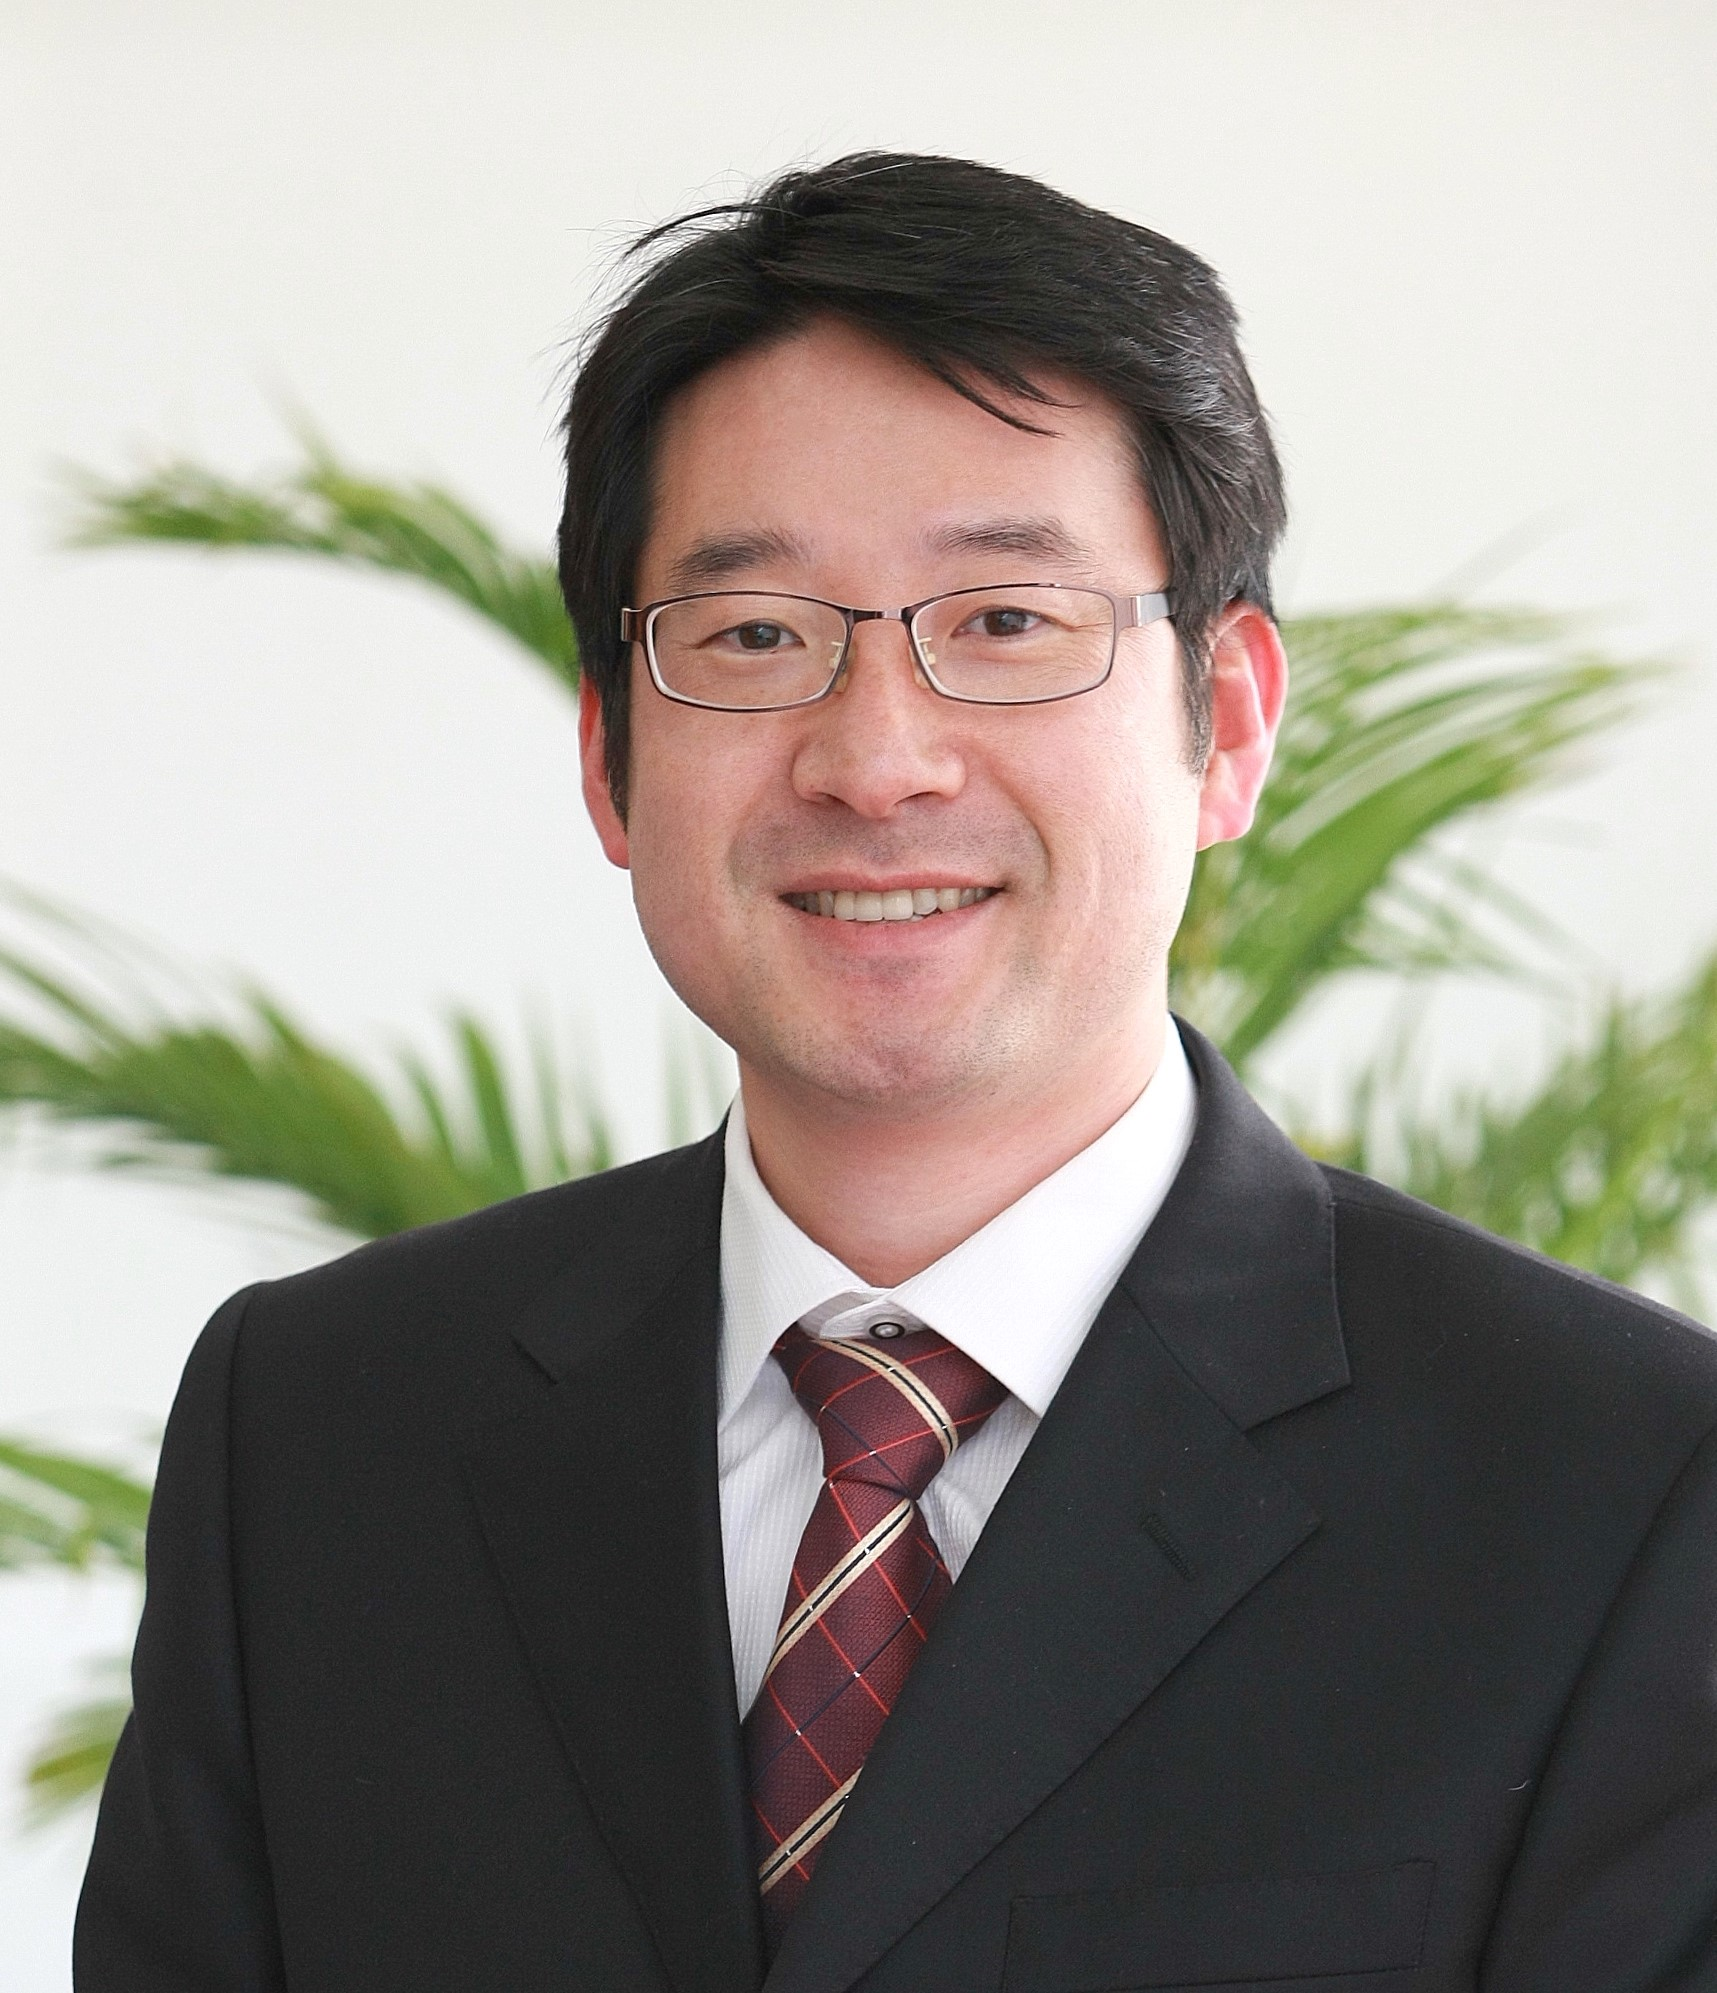
\includegraphics[width=0.2\linewidth,height=0.3\textheight]{ContributorPics/JosephKimPic} \end{center}

\begin{center}
\textbf{ Joseph H.T. Kim }
\end{center}

\begin{itemize}
\tightlist
\item
  \textbf{Joseph H.T. Kim}, Ph.D., FSA, CERA, is Associate Professor of Applied Statistics at Yonsei University, Seoul, Korea. He holds a Ph.D.~degree in Actuarial Science from the University of Waterloo, at which he taught as Assistant Professor. He also worked in the life insurance industry. He has published papers in \emph{Insurance Mathematics and Economics}, \emph{Journal of Risk and Insurance}, \emph{Journal of Banking and Finance}, \emph{ASTIN Bulletin}, and \emph{North American Actuarial Journal}, among others.
\end{itemize}

\begin{center}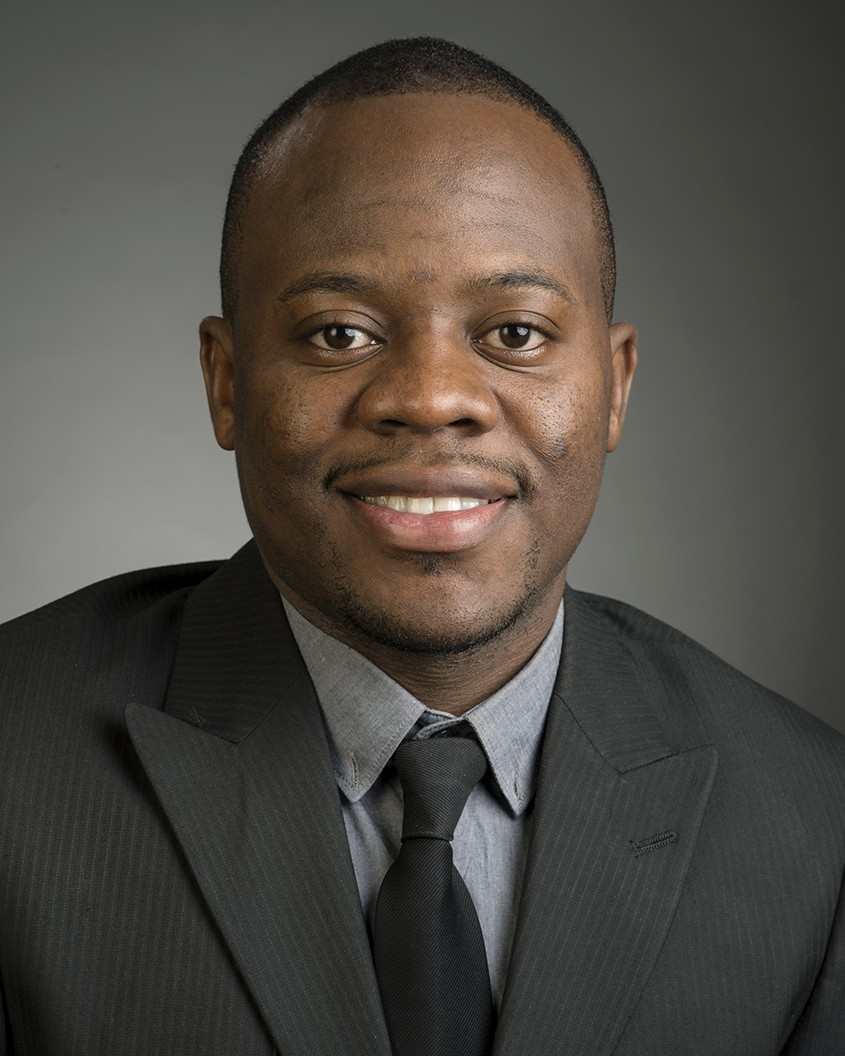
\includegraphics[width=0.2\linewidth,height=0.3\textheight]{ContributorPics/Okine_A} \end{center}

\begin{center}
\textbf{ Nii-Armah Okine }
\end{center}

\begin{itemize}
\tightlist
\item
  \textbf{Nii-Armah Okine} is an assistant professor at the Mathematical Sciences Department at Appalachian State University. He holds a Ph.D.~in Business (Actuarial Science) from the University of Wisconsin - Madison and obtained his master's degree in Actuarial science from Illinois State University. His research interest includes micro-level reserving, joint longitudinal-survival modeling, dependence modeling, micro-insurance, and machine learning.
\end{itemize}

\begin{center}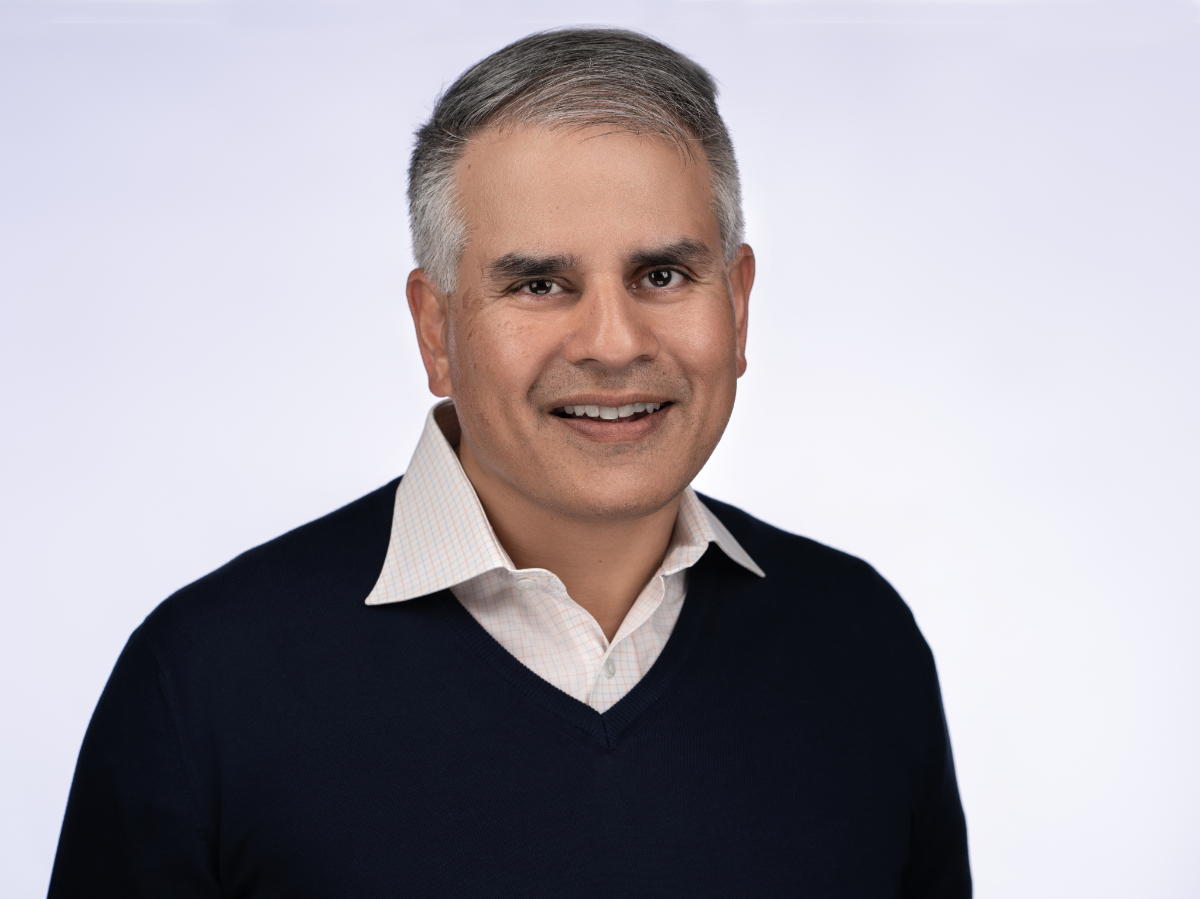
\includegraphics[width=0.3\linewidth,height=0.5\textheight]{ContributorPics/RajSahasrabuddhe} \end{center}

\begin{center}
\textbf{ Rajesh (Raj) Sahasrabuddhe }
\end{center}

\begin{itemize}
\tightlist
\item
  \textbf{Rajesh (Raj) Sahasrabuddhe} is a Partner and Philadelphia Office Leader with Oliver Wyman Actuarial Consulting. Raj is a Fellow of the Casualty Actuarial Society (CAS), an Associate of the Canadian Institute of Actuaries, and a Member of the American Academy of Actuaries. Raj has been an active volunteer with CAS Admissions committees throughout his career, including a term as Chairperson of the Syllabus Committee from 2010 to 2013. He currently serves on the MAS-II Examination Committee. He has authored or co-authored papers that have appeared on syllabi for both the CAS and Society of Actuaries.
\end{itemize}

\newpage

\begin{center}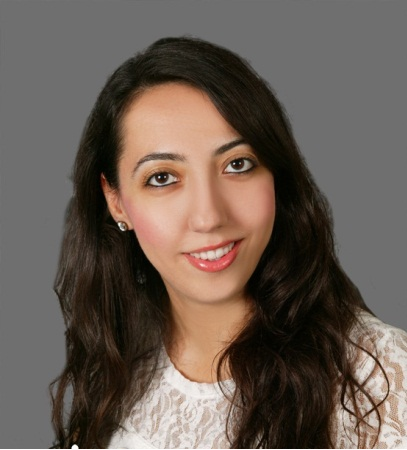
\includegraphics[width=0.2\linewidth,height=0.3\textheight]{ContributorPics/Selin_pictureA} \end{center}

\begin{center}
\textbf{ Emine Selin Sarıdaş }
\end{center}

\begin{itemize}
\tightlist
\item
  \textbf{Emine Selin Sarıdaş} is a doctoral candidate in the Statistics department of Mimar Sinan University. She holds a bachelor degree in Actuarial Science with a minor in Economics and a master degree in Actuarial Science from Hacettepe University. Her research interest includes dependence modeling, regression, loss models and life contingencies.
\end{itemize}

\begin{center}
\includegraphics[width=0.2\linewidth,height=0.3\textheight]{ContributorPics/Shi_Peng_150x188} \end{center}

\begin{center}
\textbf{ Peng Shi }
\end{center}

\begin{itemize}
\tightlist
\item
  \textbf{Peng Shi} is an associate professor in the Risk and Insurance Department at the Wisconsin School of Business. He is also the Charles \& Laura Albright Professor in Business and Finance. Professor Shi is an Associate of the Casualty Actuarial Society (ACAS) and a Fellow of the Society of Actuaries (FSA). He received a Ph.D.~in actuarial science from the University of Wisconsin-Madison. His research interests are problems at the intersection of insurance and statistics. He has won several research awards, including the Charles A. Hachemeister Prize, the Ronald Bornhuetter Loss Reserve Prize, and the American Risk and Insurance Association Prize.
\end{itemize}

\newpage

\begin{center}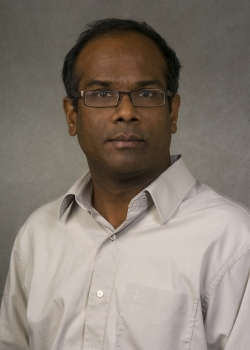
\includegraphics[width=0.2\linewidth,height=0.3\textheight]{ContributorPics/Shyamal} \end{center}

\begin{center}
\textbf{ Nariankadu D. Shyamalkumar (Shyamal) }
\end{center}

\begin{itemize}
\tightlist
\item
  \textbf{Nariankadu D. Shyamalkumar (Shyamal)} is an associate professor in the Department of Statistics and Actuarial Science at The University of Iowa. He is an Associate of the Society of Actuaries, and has volunteered in various elected and non-elected roles within the SoA. Having a broad theoretical interest as well as interest in computing, he has published in prominent actuarial, computer science, probability theory, and statistical journals. Moreover, he has worked in the financial industry, and since then served as an independent consultant to the insurance industry. He has experience educating actuaries in both Mexico and the US, serving in the roles of directing an undergraduate program, and as a graduate adviser for both masters and doctoral students.
\end{itemize}

\begin{center}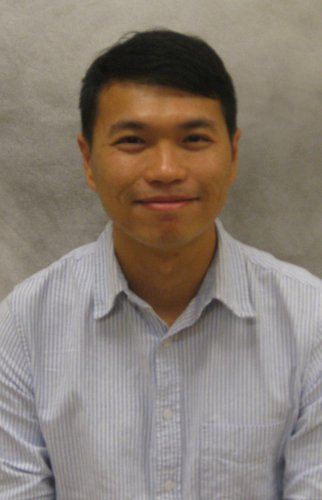
\includegraphics[width=0.2\linewidth,height=0.3\textheight]{ContributorPics/jianxi_m} \end{center}

\begin{center}
\textbf{ Jianxi Su }
\end{center}

\begin{itemize}
\tightlist
\item
  \textbf{Jianxi Su} is an Assistant Professor at the Department of Statistics at Purdue University. He is the Associate Director of Purdue's Actuarial Science. Prior to joining Purdue in 2016, he completed the PhD at York University (2012-2015). He obtained the Fellow of the Society of Actuaries (FSA) in 2017. His research expertise are in dependence modelling, risk management, and pricing. During the PhD candidature, Jianxi also worked as a research associate at the Model Validation and ORSA Implementation team of Sun Life Financial (Toronto office).
\end{itemize}

\begin{center}
\includegraphics[width=0.2\linewidth,height=0.3\textheight]{ContributorPics/ChongItTan} \end{center}

\begin{center}
\textbf{ Chong It Tan }
\end{center}

\begin{itemize}
\tightlist
\item
  \textbf{Chong It Tan} is a senior lecturer at Macquarie University in Australia, where he has served as the undergraduate actuarial program director since 2018. He obtained his PhD in 2015 from Nanyang Technological University in Singapore. He is a fully qualified actuary, holding the credentials from both the US Society of Actuaries and Australian Actuaries Institute. His major research interests are mortality modelling, longevity risk management and bonus-malus systems.
\end{itemize}

\begin{center}
\includegraphics[width=0.2\linewidth,height=0.3\textheight]{ContributorPics/TimVerdonck} \end{center}

\begin{center}
\textbf{ Tim Verdonck }
\end{center}

\begin{itemize}
\tightlist
\item
  \textbf{Tim Verdonck} is associate professor at the University of Antwerp. He has a degree in Mathematics and a PhD in Science: Mathematics, obtained at the University of Antwerp. During his PhD he successfully took the Master in Insurance and the Master in Financial and Actuarial Engineering, both at KU Leuven. His research focuses on the adaptation and application of robust statistical methods for insurance and finance data.
\end{itemize}

\newpage

\begin{center}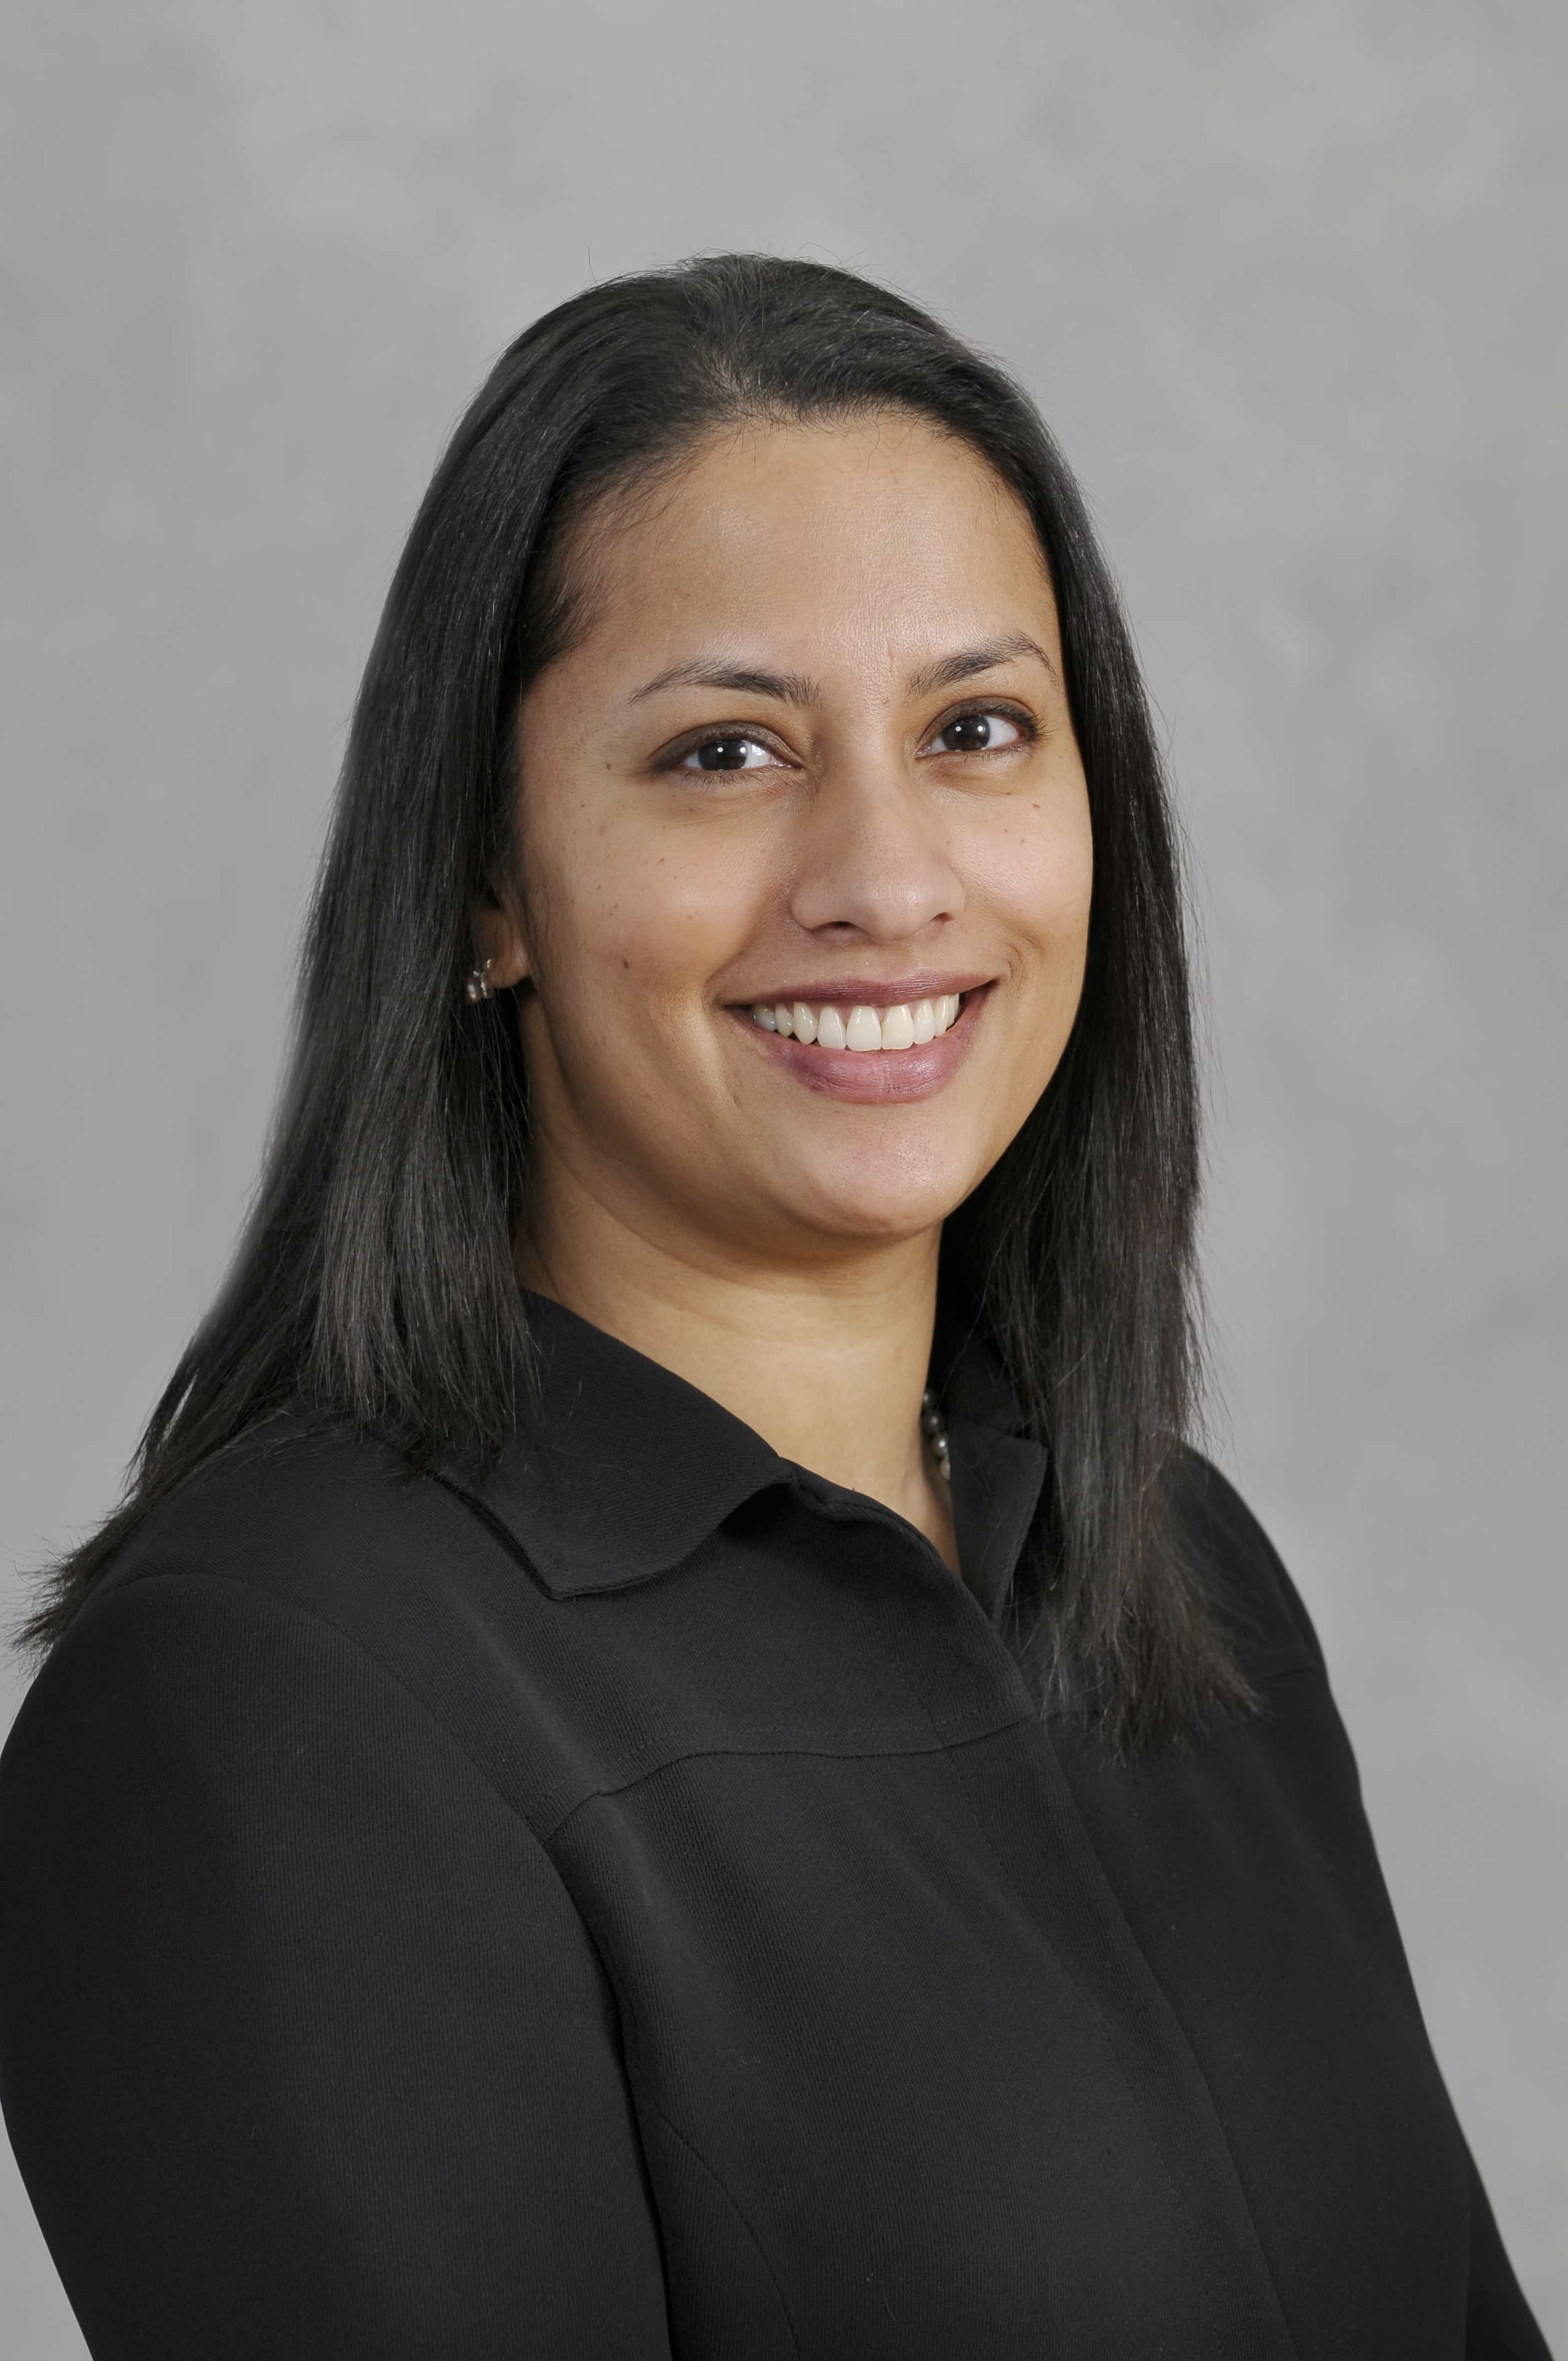
\includegraphics[width=0.2\linewidth,height=0.3\textheight]{ContributorPics/krupaviswanathan2} \end{center}

\begin{center}
\textbf{ Krupa Viswanathan }
\end{center}

\begin{itemize}
\tightlist
\item
  \textbf{Krupa Viswanathan} is an Associate Professor in the Risk, Insurance and Healthcare Management Department in the Fox School of Business, Temple University. She is an Associate of the Society of Actuaries. She teaches courses in Actuarial Science and Risk Management at the undergraduate and graduate levels. Her research interests include corporate governance of insurance companies, capital management, and sentiment analysis. She received her Ph.D.~from The Wharton School of the University of Pennsylvania.
\end{itemize}

\hypertarget{reviewers}{%
\section*{Reviewers}\label{reviewers}}


Our goal is to have the actuarial community author our textbooks in a collaborative fashion. Part of the writing process involves many reviewers who generously donated their time to help make this book better. They are:

\begin{itemize}
\tightlist
\item
  Yair Babab
\item
  David Back, Liberty Mutual
\item
  Chunsheng Ban, Ohio State University
\item
  Vytaras Brazauskas, University of Wisconsin - Milwaukee
\item
  Yvonne Chueh, Central Washington University
\item
  Chun Yong Chew, Universiti Tunku Abdul Rahman (UTAR)
\item
  Benjamin Côté, Université Laval
\item
  Eren Dodd, University of Southampton
\item
  Gordon Enderle, University of Wisconsin - Madison
\item
  Rob Erhardt, Wake Forest University
\item
  Runhun Feng, University of Illinois
\item
  Brian Hartman, Brigham Young University
\item
  Liang (Jason) Hong, University of Texas at Dallas
\item
  Fei Huang, Australian National University
\item
  Hirokazu (Iwahiro) Iwasawa
\item
  Himchan Jeong, University of Connecticut
\item
  Min Ji, Towson University
\item
  Paul Herbert Johnson, University of Wisconsin - Madison
\item
  Dalia Khalil, Cairo University
\item
  Samuel Kolins, Lebonan Valley College
\item
  Andrew Kwon-Nakamura, Zurich North America
\item
  Ambrose Lo, University of Iowa
\item
  Mélina Mailhot, Concordia University
\item
  Mark Maxwell, University of Texas at Austin
\item
  Tatjana Miljkovic, Miami University
\item
  Bell Ouelega, American University in Cairo
\item
  Zhiyu (Frank) Quan, University of Connecticut
\item
  Jiandong Ren, Western University
\item
  Margie Rosenberg, University of Wisconsin - Madison
\item
  Rajesh V. Sahasrabuddhe, Oliver Wyman
\item
  Sherly Paola Alfonso Sanchez, Universidad Nacional de Colombia
\item
  Ranee Thiagarajah, Illinois State University
\item
  Ping Wang, Saint Johns University
\item
  Chengguo Weng, University of Waterloo
\item
  Toby White, Drake University
\item
  Michelle Xia, Northern Illinois University
\item
  Di (Cindy) Xu, University of Nebraska - Lincoln
\item
  Lina Xu, Columbia University
\item
  Lu Yang, University of Amsterdam
\item
  Chun Yong
\item
  Jorge Yslas, University of Copenhagen
\item
  Jeffrey Zheng, Temple University
\item
  Hongjuan Zhou, Arizona State University
\end{itemize}

\hypertarget{other-collaborators}{%
\subsection*{Other Collaborators}\label{other-collaborators}}


\begin{itemize}
\tightlist
\item
  Alyaa Nuval Binti Othman, Aisha Nuval Binti Othman, and Khairina (Rina) Binti Ibraham were three of many students at the Univeristy of Wiscinson-Madison that helped with the text over the years.
\item
  Maggie Lee, Macquarie University, and Anh Vu (then at University of New South Wales) contributed the end of the section quizzes.
\item
  Jeffrey Zheng, Temple University, Lu Yang (University of Amsterdam), and Paul Johnson, University of Wisconsin-Madison, led the work on the glossary.
\end{itemize}

\hypertarget{version-number}{%
\section*{Version Number}\label{version-number}}


\begin{itemize}
\tightlist
\item
  This is \textbf{Version 2.0}, October 2024. Edited by Hélène Cossette, Edward (Jed) Frees, Brian Hartman, and Tim Higgins.
\item
  Version 1.1, August 2020. Edited by Edward (Jed) Frees and Paul Johnson.
\item
  Version 1.0, January 2020, was edited by Edward (Jed) Frees.
\end{itemize}

You can also access pdf and epub (current and older) versions of the text in our \href{https://ewfrees.github.io/Loss-Data-Analytics/DownloadOffline.html}{Offline versions of the text}.

\hypertarget{for-our-readers}{%
\section*{For our Readers}\label{for-our-readers}}


We hope that you find this book worthwhile and even enjoyable. For your convenience, at our \href{https://openacttexts.github.io/}{Github Landing site} (\url{https://openacttexts.github.io/}), you will find links to the book that you can (freely) download for offline reading, including a pdf version (for Adobe Acrobat) and an EPUB version suitable for mobile devices. \href{https://github.com/OpenActTexts/Loss-Data-Analytics/tree/master/Data}{Data} for running our examples are available at the same site.

In developing this book, we are emphasizing the \href{https://openacttexts.github.io/Loss-Data-Analytics/index.html}{online version} that has lots of great features such as a glossary, code and solutions to examples that you can be revealed interactively. For example, you will find that the statistical code is hidden and can only be seen by clicking on terms such as

We hide the code because we don't want to insist that you use the \texttt{R} statistical software (although we like it). Still, we encourage you to try some statistical code as you read the book -- we have opted to make it easy to learn \texttt{R} as you go. We have set up a separate \href{https://openacttexts.github.io/LDARcode}{R Code for Loss Data Analytics} site to explain more of the details of the code.

Like any book, we have a set of notations and conventions. It will probably save you time if you regularly visit our Appendix Chapter \ref{ChapNotationConvention} to get used to ours.

Freely available, interactive textbooks represent a new venture in actuarial education and we need your input. Although a lot of effort has gone into the development, we expect hiccoughs. Please let your instructor know about opportunities for improvement, write us through our project site, or contact chapter contributors directly with suggested improvements.

\begin{center}\rule{0.5\linewidth}{0.5pt}\end{center}

This work is licensed under a Creative Commons Attribution 4.0 International License.

\mainmatter

\hypertarget{ChapGlossary}{%
\chapter{Glossary}\label{ChapGlossary}}

\begin{longtable}[t]{>{\raggedright\arraybackslash}p{3cm}|>{\raggedright\arraybackslash}p{10cm}|>{\centering\arraybackslash}p{1cm}}
\hline
Term & Definition & Section\\
\hline
\endfirsthead
\multicolumn{3}{@{}l}{\textit{(continued)}}\\
\hline
Term & Definition & Section\\
\hline
\endhead
\cellcolor{gray!10}{analytics} & \cellcolor{gray!10}{Analytics is the process of using data to make decisions.} & \cellcolor{gray!10}{1.1}\\
\hline
renters insurance & Renters insurance is an insurance policy that covers the contents of an apartment or house that you are renting. & 1.1\\
\hline
\cellcolor{gray!10}{automobile insurance} & \cellcolor{gray!10}{An insurance policy that covers damage to your vehicle, damage to other vehicles in the accident, as well as medical expenses of those injured in the accident.} & \cellcolor{gray!10}{1.1}\\
\hline
casualty insurance & Causalty insurance is a form of liability insurance providing coverage for negligent acts and omissions. examples include workers compensation, errors and omissions, fidelity, crime, glass, boiler, and various malpractice coverages. & 1.1\\
\hline
\cellcolor{gray!10}{commercial insurance} & \cellcolor{gray!10}{} & \cellcolor{gray!10}{1.1}\\
\hline
term & The duration of an insurance contract & 1.1\\
\hline
\cellcolor{gray!10}{insurance claim} & \cellcolor{gray!10}{An insurance claim is the compensation provided by the insurer for incurred hurt, loss, or damage that is covered by the policy.} & \cellcolor{gray!10}{1.1}\\
\hline
homeowners insurance & Homeowners insurance is an insurance policy that covers the contents and property of a building that is owned by you or a friend. & 1.1\\
\hline
\cellcolor{gray!10}{property insurance} & \cellcolor{gray!10}{Property insurance is a policy that protects the insured against loss or damage to real or personal property. the cause of loss might be  fire, lightening, business interruption, loss of rents, glass breakage, tornado, windstorm, hail, water damage, explosion, riot, civil commotion, rain, or damage from aircraft or vehicles.} & \cellcolor{gray!10}{1.1}\\
\hline
non-life & Non-life insurance is any type of insurance where payments are not based on the death (or survivorship) of a named insured. examples include automobile, homeowners, and so on. also known as property and casualty or general insurance. & 1.1\\
\hline
\cellcolor{gray!10}{life insurance} & \cellcolor{gray!10}{Life insurance is a contract where the insurer promises to pay upon the death of an insured person. the person being paid is the beneficiary.} & \cellcolor{gray!10}{1.1}\\
\hline
personal insurance & Insurance purchased by a person & 1.1\\
\hline
\cellcolor{gray!10}{loss adjustment expenses} & \cellcolor{gray!10}{Loss adjustment expenses are costs to the insurer that are directly attributable to settling a claims. for example, the cost of an adjuster is someone who assess the claim cost or a lawyer who becomes involve in settling an insurer's legal obligation on a claim} & \cellcolor{gray!10}{1.2}\\
\hline
unallocated & Unallocated loss adjustment expenses are costs that can only be indirectly attributed to claim settlement; for example, the cost of an office to support claims staff & 1.2\\
\hline
\cellcolor{gray!10}{allocated} & \cellcolor{gray!10}{Allocated loss adjustment expenses, sometimes known by the acronym alea, are costs that can be directly attributed to settling a claim; for example, the cost of an adjuster} & \cellcolor{gray!10}{1.2}\\
\hline
underwriting & Underwriting is the process where the company makes a decision as to whether or not to take on a risk. & 1.2\\
\hline
\cellcolor{gray!10}{loss reserving} & \cellcolor{gray!10}{A loss reserve is an estimate of liability indicating the amount the insurer expects to pay for claims that have not yet been realized. this includes losses incurred but not yet reported (ibnr) and those claims that have been reported claims that haven't been paid (known by the acronym rbns for reported but not settled).} & \cellcolor{gray!10}{1.2}\\
\hline
risk classification & Risk classification is the process of grouping policyholders into categories, or classes, where each insured in the class has a risk profile that is similar to others in the class. & 1.2\\
\hline
\cellcolor{gray!10}{retrospective premiums} & \cellcolor{gray!10}{The process of determining the cost of an insurance policy based on the actual loss experience determined as an adjustment to the initial premium payment.} & \cellcolor{gray!10}{1.2}\\
\hline
claims adjustment & Claims adjustment is the process of determining coverage, legal liability, and settling claims. & 1.2\\
\hline
\cellcolor{gray!10}{claims leakage} & \cellcolor{gray!10}{Claims leakage respresents money lost through claims management inefficiencies.} & \cellcolor{gray!10}{1.2}\\
\hline
adjuster & An adjuster is a person who investigates claims and recommends settlement options based on estimates of damage and insurance policies held. & 1.2\\
\hline
\cellcolor{gray!10}{dividends} & \cellcolor{gray!10}{A dividend is the refund of a portion of the premium paid by the insured from insurer surplus.} & \cellcolor{gray!10}{1.2}\\
\hline
indemnification & Indemnification is the compensation provided by the insurer. & 1.3\\
\hline
\cellcolor{gray!10}{rating variables} & \cellcolor{gray!10}{Rating variables are the components of an insurance pricing formula. they can include numeric variables (like values, revenue, or area) and classification variables (like location, type of vehicle, or type of occupancy.)} & \cellcolor{gray!10}{1.3}\\
\hline
frequency & Count random variables that represent the number of claims & 2.1\\
\hline
\cellcolor{gray!10}{severity} & \cellcolor{gray!10}{The amount, or size, of each payment for an insured event} & \cellcolor{gray!10}{2.1}\\
\hline
probability mass function (pmf) & A function that gives the probability that a discrete random variable is exactly equal to some value & 2.1\\
\hline
\cellcolor{gray!10}{distribution function} & \cellcolor{gray!10}{The chance that the random variable is less than or equal to x, as a function of x} & \cellcolor{gray!10}{2.1}\\
\hline
mean & Average & 2.1\\
\hline
\cellcolor{gray!10}{moments} & \cellcolor{gray!10}{The rth moment of a list is the average value of the random variable raised to the rth power} & \cellcolor{gray!10}{2.1}\\
\hline
survival function & The probability that the random variable takes on a value greater than a number x & 2.1\\
\hline
\cellcolor{gray!10}{moment generating function (mgf)} & \cellcolor{gray!10}{The mgf of random variable n is defined the expectation of exp(tn), as a function of t} & \cellcolor{gray!10}{2.2}\\
\hline
probability generating function (pgf) & For a random variable n, its pgf is defined as the expectation of s\textasciicircum{}n, as a function of s & 2.2\\
\hline
\cellcolor{gray!10}{convex hulls} & \cellcolor{gray!10}{The convex hull of a set of points x is the smallest convex set that contains x} & \cellcolor{gray!10}{2.2}\\
\hline
risk classes & The formation of different premiums for the same coverage based on each homogeneous group's characteristics. & 2.2\\
\hline
\cellcolor{gray!10}{binomial distribution} & \cellcolor{gray!10}{A random variable has a binomial distribution (with parameters m and q) if it is the number of "successes" in a fixed number m of independent random trials, all of which have the same probability q of resulting in "success."} & \cellcolor{gray!10}{2.2}\\
\hline
binary outcomes & Outcomes whose unit can take on only two possible states, traditionally labeled as 0 and 1 & 2.2\\
\hline
\cellcolor{gray!10}{m-convolution} & \cellcolor{gray!10}{The addition of m independent random variables} & \cellcolor{gray!10}{2.2}\\
\hline
poisson distribution & A discrete probability distribution that expresses the probability of a given number of events occurring in a fixed interval of time or space if these events occur with a known constant rate and independently of the time since the last event & 2.2\\
\hline
\cellcolor{gray!10}{negative binomial distribution} & \cellcolor{gray!10}{The number of successes until we observe the rth failure in independent repetitions of an experiment with binary outcomes} & \cellcolor{gray!10}{2.2}\\
\hline
overdispersed & The presence of greater variability (statistical dispersion) in a data set than would be expected based on a given statistical model & 2.2\\
\hline
\cellcolor{gray!10}{underdispersed} & \cellcolor{gray!10}{There was less variation in the data than predicted} & \cellcolor{gray!10}{2.2}\\
\hline
(a, b, 0) class & The poisson, binomial and negative binomial distributions & 2.3\\
\hline
\cellcolor{gray!10}{maximum likelihood estimator (mle)} & \cellcolor{gray!10}{The possible value of the parameter for which the chance of observing the data largest} & \cellcolor{gray!10}{2.4}\\
\hline
local extrema & The largest and smallest value of the function within a given range & 2.4\\
\hline
\cellcolor{gray!10}{central limit theorem (clt)} & \cellcolor{gray!10}{In some situations, when independent random variables are added, their properly normalized sum tends toward a normal distribution even if the original variables themselves are not normally distributed.} & \cellcolor{gray!10}{2.4}\\
\hline
newton's method & A root-finding algorithm which produces successively better approximations to the roots of a real-valued function & 2.4\\
\hline
\cellcolor{gray!10}{robust} & \cellcolor{gray!10}{Resistant to errors in the results, produced by deviations from assumptions} & \cellcolor{gray!10}{2.4}\\
\hline
explanatory variables & In regression, the explanatory variable is the one that is supposed to "explain" the other. & 2.5\\
\hline
\cellcolor{gray!10}{regression analysis} & \cellcolor{gray!10}{A set of statistical processes for estimating the relationships among variables} & \cellcolor{gray!10}{2.5}\\
\hline
homogeneous & Units of exposure that face approximately the same expected frequency and severity of loss. & 2.5\\
\hline
\cellcolor{gray!10}{(a,b,1)} & \cellcolor{gray!10}{A count distribution with probabilities satisfying p\_k/p\_\{k-1\}=a+b/k, for some some constants a and b and k>=2} & \cellcolor{gray!10}{2.5}\\
\hline
zero truncation & Zero modification of a count distribution such that it assigns zero probability to zero count & 2.5\\
\hline
\cellcolor{gray!10}{degenerate distribution} & \cellcolor{gray!10}{A deterministic distribution and takes only a single value} & \cellcolor{gray!10}{2.5}\\
\hline
convex combination & A linear combination of points where all coefficients are non-negative and sum to 1 & 2.5\\
\hline
\cellcolor{gray!10}{convex function} & \cellcolor{gray!10}{A real-valued function defined on an interval is called convex if the line segment between any two points on the graph of the function lies above or on the graph.} & \cellcolor{gray!10}{2.6}\\
\hline
mixture distribution & The probability distribution of a random variable that is derived from a collection of other random variables as follows: first, a random variable is selected by chance from the collection according to given probabilities of selection, and then the value of the selected random variable is realized & 2.6\\
\hline
\cellcolor{gray!10}{chi-square distribution} & \cellcolor{gray!10}{The chi-squared distribution with k degrees of freedom is the distribution of a sum of the squares of k independent standard normal random variables} & \cellcolor{gray!10}{2.7}\\
\hline
aic & A goodness of fit measure of a statistical model that describes how well it fits a set of observations. & 2.7\\
\hline
\cellcolor{gray!10}{pearson's chi-square test} & \cellcolor{gray!10}{A statistical test applied to sets of categorical data to evaluate how likely it is that any observed difference between the sets arose by chance} & \cellcolor{gray!10}{2.7}\\
\hline
multinomial likelihood & The multinomial distribution models the probability of counts for rolling a k-sided die n times & 2.7\\
\hline
\cellcolor{gray!10}{aggregate losses} & \cellcolor{gray!10}{Aggregate claims, or total claims observed in the time period} & \cellcolor{gray!10}{3}\\
\hline
liability insurance & Insurance that compensates an insured for loss due to legal liability towards others & 3\\
\hline
\cellcolor{gray!10}{mixture distribution} & \cellcolor{gray!10}{A weighted average of other distributions, which may be continuous or discrete} & \cellcolor{gray!10}{3}\\
\hline
continuous random variable & Random variable which can take infinitely many values in its specified domain & 3.1\\
\hline
\cellcolor{gray!10}{raw moment} & \cellcolor{gray!10}{The kth moment of a random variable x is the average (expected) value of x\textasciicircum{}k} & \cellcolor{gray!10}{3.1}\\
\hline
central moment & The kth central moment of a random variable x is the expected value of (x-its mean)\textasciicircum{}k & 3.1\\
\hline
\cellcolor{gray!10}{skewness} & \cellcolor{gray!10}{Measure of the symmetry of a distribution, 3rd central moment/standard deviation\textasciicircum{}3} & \cellcolor{gray!10}{3.1}\\
\hline
kurtosis & Measure of the peaked-ness of a distribution, 4th central moment/standard deviation\textasciicircum{}4 & 3.1\\
\hline
\cellcolor{gray!10}{expected value} & \cellcolor{gray!10}{Average} & \cellcolor{gray!10}{3.1}\\
\hline
exponential distribution & A single parameter continous probability distribution that is defined by its rate parameter & 3.1\\
\hline
\cellcolor{gray!10}{independent} & \cellcolor{gray!10}{Two variables are independent if conditional information given about one variable provides no information regarding the other variable} & \cellcolor{gray!10}{3.1}\\
\hline
percentile & The pth percentile of a random variable x is the smallest value x\_p such that the probability of not exceeding it is p\% & 3.1\\
\hline
\cellcolor{gray!10}{chi-square distribution} & \cellcolor{gray!10}{A common distribution used in chi-square tests for determining goodness of fit of observed data to a theorized distribution} & \cellcolor{gray!10}{3.2}\\
\hline
light tailed distribution & A distribution with thinner tails than the benchmark exponential distribution & 3.2\\
\hline
\cellcolor{gray!10}{pareto distribution} & \cellcolor{gray!10}{A heavy-tailed and positively skewed distribution with 2 parameters} & \cellcolor{gray!10}{3.2}\\
\hline
hazard function & Ratio of the probability density function and the survival function: f(x)/s(x), and represents an instantaneous probability within a small time frame & 3.2\\
\hline
\cellcolor{gray!10}{weibull distribution} & \cellcolor{gray!10}{A positively skewed continuous distribution with 2 parameters that can have an increasing or decreasing hazard function depending on the shape parameter} & \cellcolor{gray!10}{3.2}\\
\hline
generalized beta distribution of the second kind & A 4-parameter flexible distribution that encompasses many common distributions & 3.2\\
\hline
\cellcolor{gray!10}{parametric distributions} & \cellcolor{gray!10}{Probability distribution defined by a fixed set of parameters} & \cellcolor{gray!10}{3.3}\\
\hline
transformation & A function or method that turns one distribution into another & 3.3\\
\hline
\cellcolor{gray!10}{distribution function technique} & \cellcolor{gray!10}{A transformation technique that involves finding the cdf of the transformed distribution through its relation with the original cdf} & \cellcolor{gray!10}{3.3}\\
\hline
change-of-variable technique & A transformation technique that involves finding the pdf of the transformed distribution through its relation with the original pdf using inverse functions & 3.3\\
\hline
\cellcolor{gray!10}{moment-generating function technique} & \cellcolor{gray!10}{A transformation technique that uses moment generating functions properties to determine the mgf of a linear combination of variables} & \cellcolor{gray!10}{3.3}\\
\hline
lognormal distribution & A heavy-tailed, positively skewed 2-parameter continuous distribution such that the natural log of the random variable is normally distributed with the same parameter values & 3.3\\
\hline
\cellcolor{gray!10}{reliability data} & \cellcolor{gray!10}{A dataset consisting of failure times for failed units and run times for units still functioning} & \cellcolor{gray!10}{3.3}\\
\hline
power transformation & A transformation type that involves raising a random variable to a power & 3.3\\
\hline
\cellcolor{gray!10}{exponential transformation} & \cellcolor{gray!10}{A transformation type that involves raising a random variable in the exponent} & \cellcolor{gray!10}{3.3}\\
\hline
mixing parameters & Proportion weight given to each subpopulation in a mixture & 3.3\\
\hline
\cellcolor{gray!10}{heterogeneous population} & \cellcolor{gray!10}{A dataset where the subpopulations are represented by separate distinct distributions} & \cellcolor{gray!10}{3.3}\\
\hline
finite mixture & A mixture distribution with a finite k number of subpopulations & 3.3\\
\hline
\cellcolor{gray!10}{continuous mixture} & \cellcolor{gray!10}{A mixture distribution with an infinite number of subpopulations, where the mixing parameter is itself a continuous distribution} & \cellcolor{gray!10}{3.3}\\
\hline
conditional distribution & A probability distribution that applies to a subpopulation satisfying the condition & 3.3\\
\hline
\cellcolor{gray!10}{unconditional distribution} & \cellcolor{gray!10}{A probability distribution independent of any another imposed conditions} & \cellcolor{gray!10}{3.3}\\
\hline
prior distribution & A probability distribution assigned prior to observing additional data & 3.3\\
\hline
\cellcolor{gray!10}{scale distribution} & \cellcolor{gray!10}{A distribution with the property that multiplying all values by a constant leads to the same distribution family with only the scale parameter changed} & \cellcolor{gray!10}{3.3}\\
\hline
moral hazard & Situation where an insured is more likely to be risk seeking if they do not bear sufficient consequences for a loss & 3.4\\
\hline
\cellcolor{gray!10}{payment per loss} & \cellcolor{gray!10}{Amount insurer pays when a loss occurs and can be 0} & \cellcolor{gray!10}{3.4}\\
\hline
payment per payment & Amount insurer pays given a payment is needed and is greater than 0 & 3.4\\
\hline
\cellcolor{gray!10}{left censored} & \cellcolor{gray!10}{Values below a threshold d are not ignored but converted to 0} & \cellcolor{gray!10}{3.4}\\
\hline
left truncated & Values below a threshold d are not reported and unknown & 3.4\\
\hline
\cellcolor{gray!10}{loss elimination ratio (ler)} & \cellcolor{gray!10}{\% decrease of the expected payment by the insurer as a result of the deductible} & \cellcolor{gray!10}{3.4}\\
\hline
franchise deductible & Insurer pays nothing for losses below the deductible, but pays the full amount for any loss above the deductible & 3.4\\
\hline
\cellcolor{gray!10}{limit of coverage} & \cellcolor{gray!10}{Policy limit, or maximum contractual financial obligation of the insurer for a loss} & \cellcolor{gray!10}{3.4}\\
\hline
group insurance & Insurance provided to groups of people to take advantage of lower administrative costs vs. individual policies & 3.4\\
\hline
\cellcolor{gray!10}{growth factor} & \cellcolor{gray!10}{Multiplicative factor applied to a distribution to account for the impact of inflation, typically (1+rate)} & \cellcolor{gray!10}{3.4}\\
\hline
cedent & Party that is transferring the risk to a reinsurer & 3.4\\
\hline
\cellcolor{gray!10}{excess of loss coverage} & \cellcolor{gray!10}{Contract where an insurer pays all claims up to a specified amount and then the reinsurer pays claims in excess of stated reinsurance deductible} & \cellcolor{gray!10}{3.4}\\
\hline
retention & Maximum amount payable by the primary insurer in a reinsurance arrangement & 3.4\\
\hline
\cellcolor{gray!10}{right censored variable} & \cellcolor{gray!10}{Values above a threshold u are not ignored but converted to u} & \cellcolor{gray!10}{3.4}\\
\hline
reinsurance & A transaction where the primary insurer buys insurance from a re-insurer who will cover part of the losses and/or loss adjustment expenses of the primary insurer & 3.4\\
\hline
\cellcolor{gray!10}{method of maximum likelihood} & \cellcolor{gray!10}{Statistical method used to derive the parameter values from data that maximize the probability of observing the data given the parameters} & \cellcolor{gray!10}{3.5}\\
\hline
grouped data & Data bucketed into categories with ranges, such as for use in histograms or frequency tables & 3.5\\
\hline
\cellcolor{gray!10}{large-sample properties} & \cellcolor{gray!10}{Asymptotic properties of a distribution as the amount of data increases towards infinity} & \cellcolor{gray!10}{3.5}\\
\hline
asymptotic variance & Variability of the distribution of an estimator as the amount of data increases towards infinity & 3.5\\
\hline
\cellcolor{gray!10}{delta method} & \cellcolor{gray!10}{Statistical method used to approximate the asymptotic variance for a function based on parameters whose asymptotic variance can be determined} & \cellcolor{gray!10}{3.5}\\
\hline
log-likelihood function & Natural log of the likelihood function & 3.5\\
\hline
\cellcolor{gray!10}{covariance matrix} & \cellcolor{gray!10}{Matrix where the (i,j)\textasciicircum{}th element represents the covariance between the ith and jth random variables} & \cellcolor{gray!10}{3.5}\\
\hline
complete data & Data where each individual observation is known, and no values are censored, truncated, or grouped & 3.5\\
\hline
\cellcolor{gray!10}{parametric} & \cellcolor{gray!10}{Distributional assumptions made on the population from which the data is drawn, with properties defined using parameters.} & \cellcolor{gray!10}{4.1}\\
\hline
nonparametric & No distributional assumptions are made on the population from which the data is drawn. & 4.1\\
\hline
\cellcolor{gray!10}{sampling scheme} & \cellcolor{gray!10}{How the data is obtained from the population and what data is observed.} & \cellcolor{gray!10}{4.1}\\
\hline
unbiased & An estimator that has no bias, that is, the expected value of an estimator equals the parameter being estimated. & 4.1\\
\hline
\cellcolor{gray!10}{plug-in principle} & \cellcolor{gray!10}{The plug-in principle or analog principle of estimation proposes that population parameters be estimated by sample statistics which have the same property in the sample as the parameters do in the population.} & \cellcolor{gray!10}{4.1}\\
\hline
indicator & A categorical variable that has only two groups. the numerical values are usually taken to be one to indicate the presence of an attribute, and zero otherwise. another name for a binary variable. & 4.1\\
\hline
\cellcolor{gray!10}{empirical distribution function} & \cellcolor{gray!10}{The empirical distribution is a non-parametric estimate of the underlying distribution of a random variable. it directly uses the data observations to construct the distribution, with each observed data point in a size-n sample having probability 1/n.} & \cellcolor{gray!10}{4.1}\\
\hline
first quartile & The 25th percentile; the number such that approximately 25\% of the data is below it. & 4.1\\
\hline
\cellcolor{gray!10}{third quartile} & \cellcolor{gray!10}{The 75th percentile; the number such that approximately 75\% of the data is below it.} & \cellcolor{gray!10}{4.1}\\
\hline
quantile & The q-th quantile is the point(s) at which the distribution function is equal to q, i.e. the inverse of the cumulative distribution function. & 4.1\\
\hline
\cellcolor{gray!10}{smoothed empirical quantile} & \cellcolor{gray!10}{A quantile obtained by linear interpolation between two empirical quantiles, i.e. data points.} & \cellcolor{gray!10}{4.1}\\
\hline
bandwidth & A small positive constant that defines the width of the steps and the degree of smoothing. & 4.1\\
\hline
\cellcolor{gray!10}{kernel density estimator} & \cellcolor{gray!10}{A nonparametric estimator of the density function of a random variable.} & \cellcolor{gray!10}{4.1}\\
\hline
bias-variance tradeoff & The tradeoff between model simplicity (underfitting; high bias) and flexibility (overfitting; high variance). & 4.1\\
\hline
\cellcolor{gray!10}{model diagnostics} & \cellcolor{gray!10}{Procedures to assess the validity of a model} & \cellcolor{gray!10}{4.1}\\
\hline
probability-probability (pp) plot & A plot that compares two models through their cumulative probabilities. & 4.1\\
\hline
\cellcolor{gray!10}{quantile-quantile (qq) plot} & \cellcolor{gray!10}{A plot that compares two models through their quantiles.} & \cellcolor{gray!10}{4.1}\\
\hline
goodness of fit statistics & A measure used to assess how well a statistical model fits the data, usually by summarizing the discrepancy between the observations and the expected values under the model. & 4.1\\
\hline
\cellcolor{gray!10}{goodness of fit} & \cellcolor{gray!10}{A measure used to assess how well a statistical model fits the data, usually by summarizing the discrepancy between the observations and the expected values under the model.} & \cellcolor{gray!10}{4.1}\\
\hline
method of moments & The estimation of population parameters by approximating parametric moments using empirical sample moments. & 4.1\\
\hline
\cellcolor{gray!10}{percentile matching} & \cellcolor{gray!10}{The estimation of population parameters by approximating parametric percentiles using empirical quantiles.} & \cellcolor{gray!10}{4.1}\\
\hline
percentile & A 100p-th percentile is the number such that 100 times p percent of the data is below it. & 4.1\\
\hline
\cellcolor{gray!10}{gini index} & \cellcolor{gray!10}{A measure for assessing income inequality. it measures the discrepancy between the income and population distributions and is calculated from the lorenz curve.} & \cellcolor{gray!10}{4.2}\\
\hline
model selection & The process of selecting a statistical model from a set of candidate models using data. & 4.2\\
\hline
\cellcolor{gray!10}{in-sample} & \cellcolor{gray!10}{A dataset used for analysis and model development. also known as a training dataset.} & \cellcolor{gray!10}{4.2}\\
\hline
out-of-sample & A dataset used for model validation. also known as a test dataset. & 4.2\\
\hline
\cellcolor{gray!10}{cross-validation} & \cellcolor{gray!10}{A model validation procedure in which the data sample is partitioned into subsamples, where splits are formed by separately taking each subsample as the out-of-sample dataset.} & \cellcolor{gray!10}{4.2}\\
\hline
model validation & The process of confirming that the proposed model is appropriate. & 4.2\\
\hline
\cellcolor{gray!10}{data-snooping} & \cellcolor{gray!10}{Repeatedly fitting models to a data set without a prior hypothesis of interest.} & \cellcolor{gray!10}{4.2}\\
\hline
predictive inference & Preditive inference is the process of using past data observations to predict future observations. & 4.2\\
\hline
\cellcolor{gray!10}{likelihood function} & \cellcolor{gray!10}{A function of the likeliness of the parameters in a model, given the observed data.} & \cellcolor{gray!10}{4.3}\\
\hline
ogive estimator & A nonparametric estimator for the distribution function in the presence of grouped data. & 4.3\\
\hline
\cellcolor{gray!10}{product-limit estimator} & \cellcolor{gray!10}{A nonparametric estimator of the survival function in the presence of incomplete data. also known as the kaplan-meier estimator.} & \cellcolor{gray!10}{4.3}\\
\hline
risk set & The number of observations that are active (not censored) at a specific point. & 4.3\\
\hline
\cellcolor{gray!10}{nelson-aalen} & \cellcolor{gray!10}{A nonparametric estimator of the cumulative hazard function in the presence of incomplete data.} & \cellcolor{gray!10}{4.3}\\
\hline
credibility & An actuarial method of balancing an individual's loss experience and the experience in the overall portfolio to improve ratemaking estimates. & 4.4\\
\hline
\cellcolor{gray!10}{bayesian} & \cellcolor{gray!10}{A type of statistical inference in which the model parameters and the data are random variables.} & \cellcolor{gray!10}{4.4}\\
\hline
predictive distribution & The distribution of new data, conditional on a base set of data, under the bayesian framework. & 4.4\\
\hline
\cellcolor{gray!10}{least squares} & \cellcolor{gray!10}{A technique for estimating parameters in linear regression. it is a standard approach in regression analysis to the approximate solution of overdetermined systems. in this technique, one determines the parameters that minimize the sum of squared differences between each observation and the corresponding linear combination of explanatory variables.} & \cellcolor{gray!10}{4.4}\\
\hline
markov chain monte carlo (mcmc) simulation & The class of numerical methods that use markov chains to generate draws from a posterior distribution. & 4.4\\
\hline
\cellcolor{gray!10}{improper prior} & \cellcolor{gray!10}{A prior distribution in which the sum or integral of the distribution is not finite.} & \cellcolor{gray!10}{4.4}\\
\hline
confidence interval & Another term for interval estimate. unlike a point estimate, it gives a range of reliability for approximating a parameter of interest. & 4.4\\
\hline
\cellcolor{gray!10}{decision analysis} & \cellcolor{gray!10}{Bayesian decision theory is the study of an agent's choices, which is informed by bayesian probability.} & \cellcolor{gray!10}{4.4}\\
\hline
conjugate distributions & Distributions such that the posterior and the prior come from the same family of distributions. & 4.4\\
\hline
\cellcolor{gray!10}{credibility interval} & \cellcolor{gray!10}{A summary of the posterior distribution of parameters under the bayesian framework.} & \cellcolor{gray!10}{4.4}\\
\hline
prior distribution & The distribution of the parameters prior to observing data under the bayesian framework. & 4.4\\
\hline
\cellcolor{gray!10}{exposure} & \cellcolor{gray!10}{A measure of the rating units for which rates are applied to determine the premium. for example, exposures may be measured on a per unit basis (e.g. a family with auto insurance under one contract may have an exposure of 2 cars) or per \$1,000 of value (e.g. homeowners insurance).} & \cellcolor{gray!10}{5.1}\\
\hline
inflation & Inflation is a sustained increase in the general price level of goods and services over a period of time. & 5.1\\
\hline
\cellcolor{gray!10}{business line} & \cellcolor{gray!10}{} & \cellcolor{gray!10}{5.1}\\
\hline
individual risk model & A modeling approach for aggregate losses in which the loss from each individual contract is considered. & 5.1\\
\hline
\cellcolor{gray!10}{collective risk model} & \cellcolor{gray!10}{A modeling approach for aggregate losses in which the aggregate loss is represented in terms of a frequency distribution and a severity distribution.} & \cellcolor{gray!10}{5.1}\\
\hline
coverage & Insurance coverage is the amount of risk or liability that is covered for an individual or entity by an insurance policy. & 5.1\\
\hline
\cellcolor{gray!10}{frequency distribution} & \cellcolor{gray!10}{The random number of claims that occur under the collective risk model.} & \cellcolor{gray!10}{5.1}\\
\hline
severity distribution & The randomly distributed amount of each loss under the collective risk model. & 5.1\\
\hline
\cellcolor{gray!10}{central limit theorem} & \cellcolor{gray!10}{Given certain conditions, the arithmetic mean of a large number of replications of independent random variables, each with a finite mean and variance, will be approximately normally distributed, regardless of the underlying distribution.} & \cellcolor{gray!10}{5.2}\\
\hline
term life insurance & A term life insurance policy is payable only if death of the insured occurs within a specified time, such as 5 or 10 years, or before a specified age. & 5.2\\
\hline
\cellcolor{gray!10}{pure endowment} & \cellcolor{gray!10}{A pure endowment is an insurance policy that is payable at the end of the policy period if the insured is still alive. if the insured has died, there is nothing paid in the form of benefits.} & \cellcolor{gray!10}{5.2}\\
\hline
support & The set of all outcomes for a random variable following some distribution. for example, exponentially distributed random variable x has support x>0. & 5.2\\
\hline
\cellcolor{gray!10}{convolution} & \cellcolor{gray!10}{The convolution of probability distributions is the distribution corresponding to the addition of independent random variables.} & \cellcolor{gray!10}{5.2}\\
\hline
law of iterated expectations & A decomposition of the expected value of a random variable into conditional components. specifically, for random variables x and y, e(x) = e[e(x|y)]. & 5.3\\
\hline
\cellcolor{gray!10}{compound distribution} & \cellcolor{gray!10}{A random variable follows a compound distribution if it is parameterized and contains at least one parameter that is itself a random variable. for example, the tweedie distribution is a compound distribution.} & \cellcolor{gray!10}{5.3}\\
\hline
tweedie distribution & A compound distribution that is a poisson sum of gamma random variables. because it can accommodate a discrete probability mass at zero and a continuous positive component, it is suitable for modeling aggregate insurance claims. & 5.3\\
\hline
\cellcolor{gray!10}{shape parameter} & \cellcolor{gray!10}{A numerical parameter of a parametric distribution affecting the shape of a distribution rather than simply shifting it (as a location parameter does) or stretching/shrinking it (as a scale parameter does).} & \cellcolor{gray!10}{5.3}\\
\hline
scale parameter & A numerical parameter of a parametric distribution that stretches/shrinks the distribution without changing its location or shape. the larger the scale parameter, the more spread out the distribution. the scale parameter is also the reciprocal of the rate parameter. for example, the normal distribution has scale parameter \textbackslash{}sigma. & 5.3\\
\hline
\cellcolor{gray!10}{exponential dispersion} & \cellcolor{gray!10}{A set of distributions that represents a generalisation of the natural exponential family and also plays an important role in generalized linear models.} & \cellcolor{gray!10}{5.3}\\
\hline
generalized linear models & Commonly known by the acronym glm. an extension of the linear regression model where the dependent variable is a member of the linear exponential family. glm encompasses linear, binary, count, and long-tailed, regressions all as special cases. & 5.3\\
\hline
\cellcolor{gray!10}{exponential family} & \cellcolor{gray!10}{A family of parametric distributions that are practical for modeling the underlying response variable in generalized linear models. this family includes the normal, bernoulli, poisson, and tweedie distributions as special cases, among many others.} & \cellcolor{gray!10}{5.3}\\
\hline
monte carlo simulation & A computerized statistical model that simulates the effects of various types of uncertainty. & 5.4\\
\hline
\cellcolor{gray!10}{empirical distribution} & \cellcolor{gray!10}{The empirical distribution is a non-parametric estimate of the underlying distribution of a random variable. it directly uses the data observations to construct the distribution, with each observed data point in a size-n sample having probability 1/n.} & \cellcolor{gray!10}{5.4}\\
\hline
converge & A type of stochastic convergence for a sequence of random variables x\_1,…, x\_n that approaches some other distribution as n approaches \textbackslash{}infty. & 5.4\\
\hline
\cellcolor{gray!10}{policy limits} & \cellcolor{gray!10}{A policy limit is the maximum value covered by a policy.} & \cellcolor{gray!10}{5.5}\\
\hline
ground-up loss & The total amount of loss sustained before policy adjustments are made (i.e. before deductions are applied for coinsurance, deductibles, and/or policy limits.) & 5.5\\
\hline
\cellcolor{gray!10}{per-loss basis} & \cellcolor{gray!10}{Due to policy modifications (e.g. deductibles), not all losses that occur result in payment. the per-loss basis considers every loss that occurs.} & \cellcolor{gray!10}{5.5}\\
\hline
per-payment basis & Due to policy modifications (e.g. deductibles), not all losses that occur result in payment. the per-payment basis which considers only the losses that result in some payment to the insured. & 5.5\\
\hline
\cellcolor{gray!10}{memoryless} & \cellcolor{gray!10}{The memoryless property means that a given probability distribution is independent of its history and what has already elapsed. specifically, random variable x is memoryless if pr(x > s+t | x >= s) = pr(x > t). note that it does not mean x > s+t and x >= s are independent events.} & \cellcolor{gray!10}{5.5}\\
\hline
central limit theorem & The sample mean and sample sum of a random sample of n from a population will converge to a normal curve as the sample size n grows & 6.1\\
\hline
\cellcolor{gray!10}{simulations} & \cellcolor{gray!10}{A computer generation of various hypothetical conditions and outputs, based on the model structure provided} & \cellcolor{gray!10}{6.1}\\
\hline
linear congruential generator & Algorithm that yields pseudo-randomized numbers calculated using a linear recursive relationship and a starting seed value & 6.1\\
\hline
\cellcolor{gray!10}{pseudo-random numbers} & \cellcolor{gray!10}{Values that appear random but can be replicated by formula} & \cellcolor{gray!10}{6.1}\\
\hline
inverse transform method & Samples a uniform number between 0 and 1 to represent the randomly selected percentile, then uses the inverse of the cumulative density function of the desired distribution to simulate from in order to find the simulated value from the desired distribution & 6.1\\
\hline
\cellcolor{gray!10}{quantile function} & \cellcolor{gray!10}{Inverse function for the cumulative density function which takes a percentile value in [0,1] as the input, and outputs the corresponding value in the distribution} & \cellcolor{gray!10}{6.1}\\
\hline
greatest lower bound & Largest value that is less than or equal to a specified subset of values/elements & 6.1\\
\hline
\cellcolor{gray!10}{universal life insurance} & \cellcolor{gray!10}{Type of cash value life insurance where the policy's cash value is the excess of premium payments over the cost of insurance, accumulated with interest, with adjustable premiums and coverage over time} & \cellcolor{gray!10}{6.1}\\
\hline
variable life insurance & Type of life insurance whose face value and coverage term can vary depending upon the performance of underlying invested securities & 6.1\\
\hline
\cellcolor{gray!10}{sampling variability} & \cellcolor{gray!10}{How much an estimate can vary between samples} & \cellcolor{gray!10}{6.1}\\
\hline
cauchy distribution & A continuous distribution that represents the distribution of the ratio of two independent normally random variables, where the denominator distribution has mean zero & 6.1\\
\hline
\cellcolor{gray!10}{kolmogorov-smirnov test} & \cellcolor{gray!10}{A nonparametric statistical test used to determine if a data sample could come from a hypothesized continuous probability distribution} & \cellcolor{gray!10}{6.1}\\
\hline
bootstrap & A method of sampling with replacement from the original dataset to create additional simulated datasets of the same size as the original & 6.2\\
\hline
\cellcolor{gray!10}{nonparametric approach} & \cellcolor{gray!10}{A statistical method where no assumption is made about the distribution of the population} & \cellcolor{gray!10}{6.2}\\
\hline
parametric approach & A statistical method where a prior assumption is made about the distribution or model form & 6.2\\
\hline
\cellcolor{gray!10}{bias} & \cellcolor{gray!10}{The difference between the expected value of an estimator and the parameter being estimated. bias is an estimation error that does not become smaller as one observes larger sample sizes.} & \cellcolor{gray!10}{6.2}\\
\hline
bias-corrected estimator & If an estimator is known to be consistently biased in a manner, it can be corrected using a factor to be come less biased or unbiased & 6.2\\
\hline
\cellcolor{gray!10}{jensen inequality} & \cellcolor{gray!10}{For a convex function f(x), f(expected value of x) <= expected value of f(x)} & \cellcolor{gray!10}{6.2}\\
\hline
natural estimator & An estimator that uses the sample moments as the estimators for the population & 6.2\\
\hline
\cellcolor{gray!10}{percentile bootstrap interval} & \cellcolor{gray!10}{Confidence interval for the parameter estimates determined using the actual percentile results from the bootstrap sampling approach, as every bootstrap sample has an associated parameter estimate(s) that can be ranked against the others} & \cellcolor{gray!10}{6.2}\\
\hline
k-fold cross-validation & A type of validation method where the data is randomly split into k groups, and each of the k groups is held out as a test dataset in turn, while the other k-1 gropus are used for distribution or model fitting, with the process repeated k times in total & 6.3\\
\hline
\cellcolor{gray!10}{leave-one-out cross validation} & \cellcolor{gray!10}{A special case of k-fold cross validation, where each single data point gets a turn in being the lone hold-out test data point, and n separate models in total are built and tested} & \cellcolor{gray!10}{6.3}\\
\hline
jackknife statistics & To calculate an estimator, leave out each observation in turn, calculate the sample estimator statistic each time, and average over the n separate estimates & 6.3\\
\hline
\cellcolor{gray!10}{accept-reject mechanism} & \cellcolor{gray!10}{A sampling method that is used where the random sample is discarded if not within a certain pre-specified range [a, b] and is commonly used when the traditional inverse transform method cannot be easily used} & \cellcolor{gray!10}{6.4}\\
\hline
importance sampling mechanism & Type of sampling method where values in the region of interest can be over-sampled or values outside the region of interest can be under-sampled & 6.4\\
\hline
\cellcolor{gray!10}{ergodic theorem} & \cellcolor{gray!10}{Ergodic theory studies the behavior of a dynamical system when it is allowed to run for an extended time} & \cellcolor{gray!10}{6.5}\\
\hline
markov process & A stochastic (time dependent) process that satisfies memorylessness, meaning future predictions of the process can be made solely based on its present state and not the historical path & 6.5\\
\hline
\cellcolor{gray!10}{invariant measure} & \cellcolor{gray!10}{Any mathematical measure that is preserved by a function (the mean is an example)} & \cellcolor{gray!10}{6.5}\\
\hline
composants & Component (smaller, self-contained part of larger entity) & 6.5\\
\hline
\cellcolor{gray!10}{hastings metropolis} & \cellcolor{gray!10}{A markov chain monte carlo (mcmc) method for random sampling from a probability distribution where values are iteratively generated, with the distribution of the next sample dependent only on the current sample value, and at each iteration, the candidate sample can be either accepted or rejected} & \cellcolor{gray!10}{6.5}\\
\hline
premium & Amount of money an insurer charges to provide the coverage described in the policy & 7.1\\
\hline
\cellcolor{gray!10}{ratemaking} & \cellcolor{gray!10}{Process used by insurers to calculate insurance rates, which drive insurance premiums} & \cellcolor{gray!10}{7.1}\\
\hline
insurance rates & Amount of money needed to cover losses, expenses, and profit per one unit of exposure & 7.1\\
\hline
\cellcolor{gray!10}{insured contingent event} & \cellcolor{gray!10}{A condition that results in an insurance claim} & \cellcolor{gray!10}{7.1}\\
\hline
expected costs & The cost to an insurer of payments to the insured and allocated loss adjustment expenses (alaes). overhead and profit are not included & 7.1\\
\hline
\cellcolor{gray!10}{underwriting profit} & \cellcolor{gray!10}{Profit an insurer derives from providing coverage, excluding investment income} & \cellcolor{gray!10}{7.1}\\
\hline
experience rating & A type of rating plan that uses the insured's historical loss experience as part of the premium determination & 7.1\\
\hline
\cellcolor{gray!10}{price} & \cellcolor{gray!10}{A quantity, usually of money, that is exchanged for a good or service} & \cellcolor{gray!10}{7.1}\\
\hline
rates & A rate is the price, or premium, charged per unit of exposure. a rate is a premium expressed in standardized units. & 7.1\\
\hline
\cellcolor{gray!10}{technical prices} & \cellcolor{gray!10}{} & \cellcolor{gray!10}{7.1}\\
\hline
loss cost & The sum of losses divided by an exposure; it is also known as the pure premium. & 7.2\\
\hline
\cellcolor{gray!10}{profit loading} & \cellcolor{gray!10}{A factor or percentage applied to the premium calculation to account for insurer profit in a policy} & \cellcolor{gray!10}{7.2}\\
\hline
indicated change factor & A factor calculated from the loss ratio method that calculates how the rates should change, with factors > 1 indicating an increase and vice versa & 7.2\\
\hline
\cellcolor{gray!10}{indicated rate} & \cellcolor{gray!10}{In a rate filing, the amount that the loss experience suggests that the insurer should charge to cover costs.} & \cellcolor{gray!10}{7.2}\\
\hline
credibility & Weight assigned to observed data vs. that assigned to an external or broader-based set of data & 7.4\\
\hline
\cellcolor{gray!10}{parametric distribution} & \cellcolor{gray!10}{Model assumption that the sample data comes from a population that can be modeled by a probability distribution with a fixed set of parameters} & \cellcolor{gray!10}{7.4}\\
\hline
commercial business property & Line of business that insures against damage to their buildings and contents due to a covered cause of loss & 7.4\\
\hline
\cellcolor{gray!10}{continuous variables} & \cellcolor{gray!10}{Type of variable that can take on any real value} & \cellcolor{gray!10}{7.4}\\
\hline
discrimination & Process of determining premiums on the basis of likelihood of loss. insurance laws prohibit "unfair discrimination". & 7.4\\
\hline
\cellcolor{gray!10}{rating factor} & \cellcolor{gray!10}{A rating factor, or rating variable, is a characteristic of the policyholder or risk being insured by which rates vary.} & \cellcolor{gray!10}{7.4}\\
\hline
rating variable & A rating factor, or rating variable, is a characteristic of the policyholder or risk being insured by which rates vary. & 7.4\\
\hline
\cellcolor{gray!10}{factor} & \cellcolor{gray!10}{A variable that varies by groups or categories.} & \cellcolor{gray!10}{7.4}\\
\hline
relativity & The difference of the expected risk between a specific level of a rating factor and an accepted baseline value. this difference may be arithmetic or proportional. & 7.4\\
\hline
\cellcolor{gray!10}{scale distribution} & \cellcolor{gray!10}{Suppose that y = c x, where x comes from a parametric distribution family and c is a positive constant. the distribution is said to be a scale distribution if (i) the distributions of y and x come from the same family and (ii) only a single parameter differs and that by a factor of c.} & \cellcolor{gray!10}{7.4}\\
\hline
written exposures & Exposure is based off policies written/issued & 7.5\\
\hline
\cellcolor{gray!10}{earned exposures} & \cellcolor{gray!10}{Exposure is based off amount exposed to loss for which coverage has been provided} & \cellcolor{gray!10}{7.5}\\
\hline
unearned exposures & Exposure amount for which coverage has not yet been provided & 7.5\\
\hline
\cellcolor{gray!10}{in force exposures} & \cellcolor{gray!10}{Exposure amount subject to loss at a particular point in time} & \cellcolor{gray!10}{7.5}\\
\hline
calendar year method & Experience for rating is aggregated based on calendar year, as opposed to other methods such as when a policy term began & 7.5\\
\hline
\cellcolor{gray!10}{accident date} & \cellcolor{gray!10}{Date of loss occurrence that gives rise to a claim} & \cellcolor{gray!10}{7.5}\\
\hline
report date & Date when insurer is notified of the claim & 7.5\\
\hline
\cellcolor{gray!10}{open claim} & \cellcolor{gray!10}{A claim that has been reported but not yet closed} & \cellcolor{gray!10}{7.5}\\
\hline
mix of business & Different types of policies in an insurer's portfolio & 7.5\\
\hline
\cellcolor{gray!10}{on-level earned premium} & \cellcolor{gray!10}{Earned premium of historical policies using the current rate structure} & \cellcolor{gray!10}{7.5}\\
\hline
experience loss ratio & Ratio of experience loss to on-level earned premium in the experience period & 7.5\\
\hline
\cellcolor{gray!10}{claim} & \cellcolor{gray!10}{The amount paid to an individual or corporation for the recovery, under a policy of insurance, for loss that comes within that policy.} & \cellcolor{gray!10}{7.5}\\
\hline
incurred but not reported & A claim is said to be incurred but not reported if the insured event occurs prior to a valuation date (and hence the insurer is liable for payment) but the event has not been reported to the insurer. & 7.5\\
\hline
\cellcolor{gray!10}{closed} & \cellcolor{gray!10}{A claim is said to be closed when the company deems its financial obligations on the claim to be resolved.} & \cellcolor{gray!10}{7.5}\\
\hline
valuation date & A valuation date is the date at which a company summarizes its financial position, typically quarterly or annually. & 7.5\\
\hline
\cellcolor{gray!10}{policy year} & \cellcolor{gray!10}{This is the period between a policy's anniversary dates.} & \cellcolor{gray!10}{7.5}\\
\hline
gini index & The gini index is twice the area between a lorenz curve and a 45 degree line. & 7.6\\
\hline
\cellcolor{gray!10}{line of equality} & \cellcolor{gray!10}{45 degree line equating x and y, that represents a perfect alignment in the sample and population distribution} & \cellcolor{gray!10}{7.6}\\
\hline
pp plot & Statistical plot used to assess how close a data sample matches a theorized distribution & 7.6\\
\hline
\cellcolor{gray!10}{performance curve} & \cellcolor{gray!10}{A concentration curve is a graph of the distribution of two variables, where both variables are ordered by only one of variables. for insurance applications, it is a graph of distribution of losses versus premiums, where both losses and premiums are ordered by premiums.} & \cellcolor{gray!10}{7.6}\\
\hline
community rating & This generally refers to the premium principle where all risks pay the same amount. & 7.6\\
\hline
\cellcolor{gray!10}{market conduct regulation} & \cellcolor{gray!10}{Regulation that ensures consumers obtain fair and reasonable insurance prices and coverage} & \cellcolor{gray!10}{7.7}\\
\hline
government prescribed & Government sets the entire rating system including coverages & 7.7\\
\hline
\cellcolor{gray!10}{prior approval} & \cellcolor{gray!10}{Regulator must approve rates, forms, rules filed by insurers before use} & \cellcolor{gray!10}{7.7}\\
\hline
no file & Insurers may use new rates, forms, rules without approval from regulators & 7.7\\
\hline
\cellcolor{gray!10}{file only} & \cellcolor{gray!10}{Insurers must file rates, forms, rules for record keeping and use immediately} & \cellcolor{gray!10}{7.7}\\
\hline
rating factors & Characteristics of a risk that help price the insurance contract & 8\\
\hline
\cellcolor{gray!10}{multiplicative tariff model} & \cellcolor{gray!10}{A rating method where each rating factor is the product of parameters associated with that rating factor} & \cellcolor{gray!10}{8}\\
\hline
risk characteristics & The distinguishing features of a policy that help determine the expected loss on the policy & 8.1\\
\hline
\cellcolor{gray!10}{gross insurance premium} & \cellcolor{gray!10}{Sum of expected losses and expenses and profit on a policy} & \cellcolor{gray!10}{8.1}\\
\hline
adverse selection & A pricing structure that entices riskier individuals to purchase and discourages low-risk individuals from purchasing & 8.1\\
\hline
\cellcolor{gray!10}{adverse selection spiral} & \cellcolor{gray!10}{Phenomenon where a book of business deteriorates as it attracts ever-riskier individuals when forced to increase premiums due to losses} & \cellcolor{gray!10}{8.1}\\
\hline
a priori variables & Variables which the insurer has prior knowledge of before the policy inception & 8.1\\
\hline
\cellcolor{gray!10}{closed-form expressions} & \cellcolor{gray!10}{A mathematical expression that can be well defined with a formula that has a finite number of operations} & \cellcolor{gray!10}{8.2}\\
\hline
levels & Different outcomes of a categorical variable & 8.2\\
\hline
\cellcolor{gray!10}{nominal} & \cellcolor{gray!10}{A categorical variable where the categories do not have a natural order and any numbering is arbitrary} & \cellcolor{gray!10}{8.2}\\
\hline
dummy variables & A variable that takes on a value of 0 or 1 to indicate the absence or presence of a categorical characteristic & 8.2\\
\hline
\cellcolor{gray!10}{log linear form} & \cellcolor{gray!10}{Linear regression model where the response variable is the natural log of the expected response value} & \cellcolor{gray!10}{8.2}\\
\hline
base case & The categorical level chosen as the default with all dummy variable indicators of 0 & 8.2\\
\hline
\cellcolor{gray!10}{workers compensation} & \cellcolor{gray!10}{A no-fault insurance system prescribed by state law where benefits are provided by an employer to an employee due to a job-related injury, including death, resulting from an accident or occupational disease} & \cellcolor{gray!10}{8.2}\\
\hline
exposure bases & The unit of measurement chosen to represent the exposure for a particular risk & 8.2\\
\hline
\cellcolor{gray!10}{offset} & \cellcolor{gray!10}{Natural log of the exposure amount that is added to a regression model to account for varying exposures} & \cellcolor{gray!10}{8.2}\\
\hline
tariff & A table or list that contains the rating factors and associated premiums and other risk information & 8.3\\
\hline
\cellcolor{gray!10}{in-force times} & \cellcolor{gray!10}{The timeframe during which a policy is active and the insurer is bound by the contractual obligation} & \cellcolor{gray!10}{8.3}\\
\hline
rate parameter & Parameter in certain distributions, such as the exponential, that indicate how quickly the function decays, and it is the reciprocal of the scale parameter & 8.3\\
\hline
\cellcolor{gray!10}{functional forms} & \cellcolor{gray!10}{The algebraic relationship between a dependent variable and explanatory variables} & \cellcolor{gray!10}{8.3}\\
\hline
multiplicative form & Relationship where the dependent variable is a product of the explanatory variables & 8.3\\
\hline
\cellcolor{gray!10}{base tariff cell} & \cellcolor{gray!10}{The chosen set of rating categories where the rate equals the intercept of the model (the base value)} & \cellcolor{gray!10}{8.3}\\
\hline
relativities & A numerical estimate of value in one category relative to the value in a base classification, typically expressed as a factor & 8.3\\
\hline
\cellcolor{gray!10}{non-automobile vehicles} & \cellcolor{gray!10}{Motorized vehicles which are not autos, such as atvs, off-road vehicles, go-carts, etc.} & \cellcolor{gray!10}{8.3}\\
\hline
distributional structure & The manner in which a statistical distribution is parameterized & 8.3\\
\hline
\cellcolor{gray!10}{information matrix} & \cellcolor{gray!10}{Matrix that measures the amount of information that an observable random variable x carries about an unknown parameter of a distribution, and is used to calculate covariance matrices of maximum likelihood estimators} & \cellcolor{gray!10}{8.5}\\
\hline
classification rating plan & A rating plan that uses an insured's risk characteristics to determine premium & 9.1\\
\hline
\cellcolor{gray!10}{credibility weight} & \cellcolor{gray!10}{The weight assigned to an insured's historical loss experience for the purposes of determining their premium in an experience rating plan} & \cellcolor{gray!10}{9.1}\\
\hline
complement of credibility & The remainder of the weight not assigned to an insured's historical loss experience in the experience rating plan & 9.1\\
\hline
\cellcolor{gray!10}{class rate} & \cellcolor{gray!10}{Average rate per exposure for an insured in a particular classification group} & \cellcolor{gray!10}{9.1}\\
\hline
full credibility standard & The threshold of experience necessary to assign 100\% credibility to the insured's own experience & 9.2\\
\hline
\cellcolor{gray!10}{limited fluctuation credibility} & \cellcolor{gray!10}{A credibility method that attempts to limit fluctuations in its estimates} & \cellcolor{gray!10}{9.2}\\
\hline
cumulative distribution function of the standard normal & Cumulative density function for the normal distribution with mean 0 and standard deviation 1 & 9.2\\
\hline
\cellcolor{gray!10}{buhlmann credibility} & \cellcolor{gray!10}{A credibility method that uses the amount of experience, expected value of the process variance, and variance of the hypothetical means to determine the credibility weight} & \cellcolor{gray!10}{9.3}\\
\hline
collective mean & The mean estimate of a risk when no loss information about the risk is known & 9.3\\
\hline
\cellcolor{gray!10}{law of total expectation} & \cellcolor{gray!10}{The expected value of the conditional expected value of x given y is the same as the expected value of x} & \cellcolor{gray!10}{9.3}\\
\hline
risk parameter & Parameter in a distribution whose value reflects the risk categorization & 9.3\\
\hline
\cellcolor{gray!10}{expected value of the process variance} & \cellcolor{gray!10}{Average of the natural variability of observations from within each risk} & \cellcolor{gray!10}{9.3}\\
\hline
variance of the hypothetical means & Variance of the means across different classes, used to determine how similar or different the classes are from one another & 9.3\\
\hline
\cellcolor{gray!10}{buhlmann-straub credibility} & \cellcolor{gray!10}{An extension of the buhlmann credibility model that allows for varying exposure by year} & \cellcolor{gray!10}{9.4}\\
\hline
bayes theorem & A probability law that expresses conditional probability of the event a given the event b in terms of the conditional probability of the event b given the event a and the unconditional probability of a & 9.5\\
\hline
\cellcolor{gray!10}{bayesian inference} & \cellcolor{gray!10}{A branch of statistics that leverages bayes theorem to update the distribution as more experience becomes available} & \cellcolor{gray!10}{9.5}\\
\hline
gamma-poisson model & A statistical model that assumes the frequency of claims is poisson whose mean has a prior distribution that is a gamma distribution & 9.5\\
\hline
\cellcolor{gray!10}{exact credibility} & \cellcolor{gray!10}{A situation where the bayesian credibility estimate matches that of the buhlmann credibility estimate} & \cellcolor{gray!10}{9.5}\\
\hline
beta-binomial model & A statistical model for modeling the probability of an event using the binomial distribution with a probability that has a prior distribution from a beta distribution & 9.5\\
\hline
\cellcolor{gray!10}{nonparametric estimation} & \cellcolor{gray!10}{Statistical method that allows the functional form of a fit from data to have no assumed prior distribution, constraints, or parameters} & \cellcolor{gray!10}{9.5}\\
\hline
empirical bayes methods & Credibility methods that estimate the credibility weight without using any assumptions about prior distributions or likelihoods, instead relying only on empirical data & 9.5\\
\hline
\cellcolor{gray!10}{semiparametric estimation} & \cellcolor{gray!10}{Credibility method that assumes a distribution for the loss per exposure random variable and otherwise uses empirical data} & \cellcolor{gray!10}{9.5}\\
\hline
portfolios & A collection of contracts & 10.1\\
\hline
\cellcolor{gray!10}{insurance portfolios} & \cellcolor{gray!10}{A collection, or aggregation, of insurance contracts} & \cellcolor{gray!10}{10.1}\\
\hline
reinsurers & A company that sells reinsurance & 10.1\\
\hline
\cellcolor{gray!10}{heavy tailed} & \cellcolor{gray!10}{A rv is said to be heavy tailed if high probabilities are assigned to large values} & \cellcolor{gray!10}{10.2}\\
\hline
survival function & One minus the distribution function. it gives the probability that a rv exceeds a specific value. & 10.2\\
\hline
\cellcolor{gray!10}{coherent risk measure} & \cellcolor{gray!10}{A risk measure that is is subadditive, monontonic, has positive homogeneity, and is translation invariant.} & \cellcolor{gray!10}{10.3}\\
\hline
mean excess loss function & The expected value of a loss in excess of a quantity, given that the loss exceeds the quantity & 10.3\\
\hline
\cellcolor{gray!10}{risk measure} & \cellcolor{gray!10}{A measure that summarizes the riskiness, or uncertainty, of a distribution} & \cellcolor{gray!10}{10.3}\\
\hline
value-at-risk & A risk measure based on a quantile function & 10.3\\
\hline
\cellcolor{gray!10}{ceding company} & \cellcolor{gray!10}{A company that purchases reinsurance (also known as the reinsured)} & \cellcolor{gray!10}{10.4}\\
\hline
excess of loss & Under an excess of loss arrangement, the insurer sets a retention level for each claim and pays claim amounts less than the level with the reinsurer paying the excess. & 10.4\\
\hline
\cellcolor{gray!10}{primary insurance} & \cellcolor{gray!10}{Insurance purchased by a non-insurer} & \cellcolor{gray!10}{10.4}\\
\hline
proportional reinsurance & An agreement between a reinsurer and a ceding company (also known as the reinsured) in which the reinsurer assumes a given percent of losses and premium & 10.4\\
\hline
\cellcolor{gray!10}{quota share} & \cellcolor{gray!10}{A proportional treaty where the reinsurer receives a flat percent of the premium for the book of business reinsured and pays a percentage of losses, including allocated loss adjustment expenses. the reinsurer may also pays the ceding company a ceding commission which is designed to reflect the differences in underwriting expenses incurred.} & \cellcolor{gray!10}{10.4}\\
\hline
reinsured & A company that purchases reinsurance (also known as the ceding company) & 10.4\\
\hline
\cellcolor{gray!10}{retained line} & \cellcolor{gray!10}{The amount of exposure that the the reinsured retains on a given line in a surplus share reinsurance agreement.} & \cellcolor{gray!10}{10.4}\\
\hline
retention function & A function that maps the insurer portfolio loss into the amount of loss retained by the insurer. & 10.4\\
\hline
\cellcolor{gray!10}{stop-loss} & \cellcolor{gray!10}{Under a stop-loss arrangement, the insurer sets a retention level and pays in full total claims less than the level with the reinsurer paying the excess.} & \cellcolor{gray!10}{10.4}\\
\hline
surplus share & A proportional reinsurance treaty that is common in commercial property insurance. a surplus share treaty allows the reinsured to limit its exposure on any one risk to a given amount (the retained line). the reinsurer assumes a part of the risk in proportion to the amount that the insured value exceeds the retained line, up to a given limit (expressed as a multiple of the retained line, or number of lines). & 10.4\\
\hline
\cellcolor{gray!10}{treaty} & \cellcolor{gray!10}{A reinsurance contract that applies to a designated book of business or exposures.} & \cellcolor{gray!10}{10.4}\\
\hline
bonus-malus system & A type of rating mechanism where insured premiums are adjusted based on their individual loss experience history & 12.1\\
\hline
\cellcolor{gray!10}{no claim discount (ncd) system} & \cellcolor{gray!10}{A type of experience rating where insureds obtain discounts on future years' premiums based on claims-free experience} & \cellcolor{gray!10}{12.1}\\
\hline
hunger for bonus & Phenomenon where insureds under an experience rating system are dissuaded from filing minor claims in order to keep their no-claims discount & 12.1\\
\hline
\cellcolor{gray!10}{takaful} & \cellcolor{gray!10}{Co-operative system of reimbursement or repayment in case of loss as an insurance alternative} & \cellcolor{gray!10}{12.2}\\
\hline
markov chain & A stochastic model (time dependent) where the probability of each event depends only on the current state and not the historical path & 12.3\\
\hline
\cellcolor{gray!10}{transition matrix} & \cellcolor{gray!10}{Matrix that represents all probabilities for transition from one state to another (could be same state) for a markov chain} & \cellcolor{gray!10}{12.3}\\
\hline
stationary distribution & Probability distribution remains unchanged in the markov chain as time progresses & 12.4\\
\hline
\cellcolor{gray!10}{ergodic} & \cellcolor{gray!10}{Irreducible markov chain where it is eventually possible to move from any state to any other state, with positive probability} & \cellcolor{gray!10}{12.4}\\
\hline
irreversible & A markov chain where there does not exist a probability distribution that allows for the chain to be walked backwards in time & 12.4\\
\hline
\cellcolor{gray!10}{eigenvector} & \cellcolor{gray!10}{A non-zero vector that changes by only a scalar factor when that linear transformation is applied} & \cellcolor{gray!10}{12.4}\\
\hline
n-step transition probability & Probability of ending in a state j after n periods, starting in state i, where i and j can be the same state & 12.4\\
\hline
\cellcolor{gray!10}{convergence rate} & \cellcolor{gray!10}{After n transitions, the sum of variation between the probability in each state vs. the stationary probability} & \cellcolor{gray!10}{12.4}\\
\hline
poisson regression model & Type of regression model used for fitting data with an integral (count) response variable with mean equal to the variance & 12.5\\
\hline
\cellcolor{gray!10}{negative binomial regression model} & \cellcolor{gray!10}{Type of regression model used for fitting data with an integral (count) response variable and can account for variance greater than the mean} & \cellcolor{gray!10}{12.5}\\
\hline
overdispersion & Phenomenon where the variance of data is larger than what is modeled & 12.5\\
\hline
\cellcolor{gray!10}{cross-classified rating classes} & \cellcolor{gray!10}{Table that combines the effects of multiple rating classifications} & \cellcolor{gray!10}{12.5}\\
\hline
structured data & Data that can be organized into a repository format, typically a database & 13.1\\
\hline
\cellcolor{gray!10}{unstructured data} & \cellcolor{gray!10}{Data that is not in a predefined format, most notably text, audio visual} & \cellcolor{gray!10}{13.1}\\
\hline
qualitative data & Data which is non numerical in nature & 13.1\\
\hline
\cellcolor{gray!10}{quantitative data} & \cellcolor{gray!10}{Data which is numerical in nature} & \cellcolor{gray!10}{13.1}\\
\hline
ordinal data & Data field with a natural ordering & 13.1\\
\hline
\cellcolor{gray!10}{interval data} & \cellcolor{gray!10}{Continuous data which is broken into interval bands with a natural ordering} & \cellcolor{gray!10}{13.1}\\
\hline
key-value databases & Data storage method that stores amd finds records using a unique key hash & 13.1\\
\hline
\cellcolor{gray!10}{column-oriented databases} & \cellcolor{gray!10}{Data storage method that stores records by column instead of by row} & \cellcolor{gray!10}{13.1}\\
\hline
document databases & Data storage method that uses the document metadata for search and retrieval, also known as semi-structured data & 13.1\\
\hline
\cellcolor{gray!10}{data decay} & \cellcolor{gray!10}{Corruption of data due to hardware failure in the storage device} & \cellcolor{gray!10}{13.1}\\
\hline
reverification & Manual process of checking the integrity of data & 13.1\\
\hline
\cellcolor{gray!10}{data element analysis} & \cellcolor{gray!10}{Analysis of the format and definition of each field} & \cellcolor{gray!10}{13.1}\\
\hline
structural analysis & Statistical analysis of the structured data present to detect irregularities & 13.1\\
\hline
\cellcolor{gray!10}{robust} & \cellcolor{gray!10}{Statistics which are more unaffected by outliers or small departures from model assumptions} & \cellcolor{gray!10}{13.2}\\
\hline
exploratory data analysis & Approach to analyzing data sets to summarize their main characteristics, using visual methods, descriptive statistics, clustering, dimension reduction & 13.2\\
\hline
\cellcolor{gray!10}{confirmatory data analysis} & \cellcolor{gray!10}{Process used to challenge assumptions about the data through hypothesis tests, significance testing, model estimation, prediction, confidence intervals, and inference} & \cellcolor{gray!10}{13.2}\\
\hline
supervised learning methods & Model that predicts a response target variable using explanatory predictors as input & 13.2\\
\hline
\cellcolor{gray!10}{unsupervised learning methods} & \cellcolor{gray!10}{Models that work with explanatory variables only to describe patterns or groupings} & \cellcolor{gray!10}{13.2}\\
\hline
classification methods & Supervised learning method where the response is a categorical variable & 13.2\\
\hline
\cellcolor{gray!10}{regression methods} & \cellcolor{gray!10}{Classical supervised learning method where the response may be continuous, binary, or a mixture of discrete and continuous} & \cellcolor{gray!10}{13.2}\\
\hline
model flexibility & A measure of model complexity, typically based on the number of estimated parameters & 13.2\\
\hline
\cellcolor{gray!10}{explanatory modeling} & \cellcolor{gray!10}{Process where the modeling goal is to identify variables with meaningful and statistically significant relationships and test hypotheses} & \cellcolor{gray!10}{13.2}\\
\hline
predictive modeling & Process where the modeling goal is to predict new observations & 13.2\\
\hline
\cellcolor{gray!10}{data modeling} & \cellcolor{gray!10}{Assumes data generated comes from a stochastic data model} & \cellcolor{gray!10}{13.2}\\
\hline
algorithmic modeling & Assumes data generated comes from unknown algorithmic models & 13.2\\
\hline
\cellcolor{gray!10}{predictive accuracy} & \cellcolor{gray!10}{Quantitative measure of how well the explanatory variables predict the response outcome} & \cellcolor{gray!10}{13.2}\\
\hline
scripts & A program or sequence of instructions that is executed by another program & 13.2\\
\hline
\cellcolor{gray!10}{reproducible analysis} & \cellcolor{gray!10}{Modeling practice where data, code, analyses are published together in a manner so that others may verify the findings} & \cellcolor{gray!10}{13.2}\\
\hline
literate programming & Coding practice where documentation and code are written together & 13.2\\
\hline
\cellcolor{gray!10}{data ownership} & \cellcolor{gray!10}{Governance process that details legal ownership of enterprise-wide data and outlines who has ability to create, edit, modify, share and restrict access to the data} & \cellcolor{gray!10}{13.2}\\
\hline
machine learning & Study of algorithms and statistical models that perform a specific task without using explicit instructions, relying on patterns and inference & 13.3\\
\hline
\cellcolor{gray!10}{pattern recognition} & \cellcolor{gray!10}{Automated recognition of patterns and regularities in data} & \cellcolor{gray!10}{13.3}\\
\hline
data mining & Process of collecting, cleaning, processing, analyzing, and discovering patterns and useful insights from large data sets & 13.3\\
\hline
\cellcolor{gray!10}{principal component analysis} & \cellcolor{gray!10}{Dimension reduction technique that uses orthogonal transformations to convert a set of possibly correlated variables into a set of linearly uncorrelated variables} & \cellcolor{gray!10}{13.3}\\
\hline
cluster analysis & Unsupervised learning method that aims to splot data into homogenous groups using a similarity measure & 13.3\\
\hline
\cellcolor{gray!10}{k-means algorithm} & \cellcolor{gray!10}{Type of clustering that aims to partition data into k mutually exclusive clusters by assigning observations to the cluster with the nearest centroid} & \cellcolor{gray!10}{13.3}\\
\hline
linear regression & Supervised model that uses a linear function to approximate the relationship between the target and explanatory variables & 13.3\\
\hline
\cellcolor{gray!10}{generalized linear model} & \cellcolor{gray!10}{Supervised model that generalizes linear regression by allowing the linear component to be related to the response variable via a link function and by allowing the variance of each measurement to be a function of its predicted value} & \cellcolor{gray!10}{13.3}\\
\hline
systematic component & The linear combination of explanatory variables component in a glm & 13.3\\
\hline
\cellcolor{gray!10}{link function} & \cellcolor{gray!10}{Function that relates between the linear predictor component to the mean of the target variable} & \cellcolor{gray!10}{13.3}\\
\hline
decision trees & Modeling technique that uses a tree-like model of decisions to divide the sample space into non-overlapping regions to make predictions & 13.3\\
\hline
\cellcolor{gray!10}{categorical variable} & \cellcolor{gray!10}{A variable whose values are qualitative groups and can have no natural ordering (nominal) or an ordering (ordinal)} & \cellcolor{gray!10}{14.1}\\
\hline
variables & A variable is any characteristics, number, or quantity that can be measured or counted. & 14.1\\
\hline
\cellcolor{gray!10}{interval variable} & \cellcolor{gray!10}{An ordinal variable with the additional property that the magnitudes of the differences between two values are meaningful} & \cellcolor{gray!10}{14.1}\\
\hline
spatial data & Data and information having an implicit or explicit association with a location relative to the earth & 14.1\\
\hline
\cellcolor{gray!10}{high dimensional} & \cellcolor{gray!10}{Data set is high dimensional when it has many variables. In many applications, the number of variables may be larger than the sample size.} & \cellcolor{gray!10}{14.1}\\
\hline
qualitative & This is a type of variable in which the measurement denotes membership in a set of groups, or categories & 14.1\\
\hline
\cellcolor{gray!10}{nominal variable} & \cellcolor{gray!10}{This is a type of qualitative/ categorical variable which has two or more categories without having any kind of natural order.} & \cellcolor{gray!10}{14.1}\\
\hline
ordinal variable & This is a type of qualitative/ categorical variable which has two or more ordered categories. & 14.1\\
\hline
\cellcolor{gray!10}{binary variable} & \cellcolor{gray!10}{Is a special type of categorical variable where there are only two categories.} & \cellcolor{gray!10}{14.1}\\
\hline
quantitative variable & A quantitative variable is a type of variable in which numerical level is a realization from some scale so that the distance between any two levels of the scale takes on meaning. & 14.1\\
\hline
\cellcolor{gray!10}{continuous variable} & \cellcolor{gray!10}{A continuous variable is a quantitative variable that can take on any value within a finite interval.} & \cellcolor{gray!10}{14.1}\\
\hline
policyholder & Person in actual possession of insurance policy; policy owner. & 14.1\\
\hline
\cellcolor{gray!10}{discrete variable} & \cellcolor{gray!10}{A discrete variable is quantitative variable that takes on only a finite number of values in any finite interval.} & \cellcolor{gray!10}{14.1}\\
\hline
count variable & A count variable is a discrete variable with values on nonnegative integers. & 14.1\\
\hline
\cellcolor{gray!10}{circular data} & \cellcolor{gray!10}{In a circular data, all values around the circle are equally likely. Example, imagine an analog picture of a clock.} & \cellcolor{gray!10}{14.1}\\
\hline
insurers & An insurance company authorized to write insurance under the laws of any state. & 14.1\\
\hline
\cellcolor{gray!10}{multivariate} & \cellcolor{gray!10}{Multivariate variable involves taking many measurements on a single entity.} & \cellcolor{gray!10}{14.1}\\
\hline
workers compensation & Insurance that covers an employer's liability for injuries, disability or death to persons in their employment, without regard to fault, as prescribed by state or federal workers' compensation laws and other statutes. & 14.1\\
\hline
\cellcolor{gray!10}{univariate} & \cellcolor{gray!10}{Univariate analysis is the simplest form of analyzing data. “Uni” means “one”, so in other words your data has only one variable.} & \cellcolor{gray!10}{14.1}\\
\hline
missing data & Missing data occur when no data value is stored for a variable in an observation. Missing data can occur because of nonresponse: no information is provided for one or more items or for a whole unit or subject. & 14.1\\
\hline
\cellcolor{gray!10}{censored} & \cellcolor{gray!10}{Censored data have unknown values beyond a bound on either end of the number line or both. Here, the data is observed but the values (measurements) are not known completely.} & \cellcolor{gray!10}{14.1}\\
\hline
truncated & Truncation occurs when values beyond a boundary are either excluded when gathered or excluded when analyzed. An object can be detected only if its value is greater than some number. & 14.1\\
\hline
\cellcolor{gray!10}{stochastic process} & \cellcolor{gray!10}{Stochastic process is defined as a collection of random variables that is indexed by some mathematical set, meaning that each random variable of the stochastic process is uniquely associated with an element in the set.} & \cellcolor{gray!10}{14.1}\\
\hline
deductibles & A deductible is a parameter specified in the contract. Typically, losses below the deductible are paid by the policyholder whereas losses in excess of the deductible are the insurer's responsibility (subject to policy limits and coninsurance). & 14.1\\
\hline
\cellcolor{gray!10}{rank based measures} & \cellcolor{gray!10}{Statistical dependence between the rankings of two variables} & \cellcolor{gray!10}{14.2}\\
\hline
odds ratio & A statistic quantifying the strength of the association between two events, a and b, which is defined as the ratio of the odds of a in the presence of b and the odds of a in the absence of b & 14.2\\
\hline
\cellcolor{gray!10}{likelihood ratio test} & \cellcolor{gray!10}{A statistical test of the goodness-of-fit between two models} & \cellcolor{gray!10}{14.2}\\
\hline
pearson correlation & A measure of the linear correlation between two variables & 14.2\\
\hline
\cellcolor{gray!10}{product-moment (pearson) correlation} & \cellcolor{gray!10}{Pearson correlation, a measure of the linear correlation between two variables} & \cellcolor{gray!10}{14.2}\\
\hline
kendall tau & A statistic used to measure the ordinal association between two measured quantities & 14.2\\
\hline
\cellcolor{gray!10}{concordant} & \cellcolor{gray!10}{An observation pair (x,y) is said to be concordant if the observation with a larger value of x has also the larger value of y} & \cellcolor{gray!10}{14.2}\\
\hline
discordant & An observation pair (x,y) is said to be discordant if the observation with a larger value of x has the smaller value of y & 14.2\\
\hline
\cellcolor{gray!10}{pearson chi-square statistic} & \cellcolor{gray!10}{A statistical test applied to sets of categorical data to evaluate how likely it is that any observed difference between the sets arose by chance} & \cellcolor{gray!10}{14.2}\\
\hline
tetrachoric correlation & A technique for estimating the correlation between two theorised normally distributed continuous latent variables, from two observed binary variables & 14.2\\
\hline
\cellcolor{gray!10}{polychoric correlation} & \cellcolor{gray!10}{A technique for estimating the correlation between two theorised normally distributed continuous latent variables, from two observed ordinal variables} & \cellcolor{gray!10}{14.2}\\
\hline
polyserial correlation & The correlation between two continuous variables with a bivariate normal distribution, where one variable is observed directly, and the other is unobserved & 14.2\\
\hline
\cellcolor{gray!10}{biserial correlation} & \cellcolor{gray!10}{A correlation coefficient used when one variable is dichotomous} & \cellcolor{gray!10}{14.2}\\
\hline
normal score & Transformed data which closely resemble a standard normal distribution & 14.2\\
\hline
\cellcolor{gray!10}{copula} & \cellcolor{gray!10}{A multivariate distribution function with uniform marginals} & \cellcolor{gray!10}{14.3}\\
\hline
spearmans rho & A nonparametric measure of rank correlation & 14.3\\
\hline
\cellcolor{gray!10}{marginal distributions} & \cellcolor{gray!10}{The probability distribution of the variables contained in the subset of a collection of random variables} & \cellcolor{gray!10}{14.4}\\
\hline
fat-tailed & A fat-tailed distribution is a probability distribution that exhibits a large skewness or kurtosis, relative to that of either a normal distribution or an exponential distribution & 14.4\\
\hline
\cellcolor{gray!10}{probability integral transformation} & \cellcolor{gray!10}{Any continuous variable can be mapped to a uniform random variable via its distribution function} & \cellcolor{gray!10}{14.4}\\
\hline
elliptical copulas & The copulas of elliptical distributions & 14.5\\
\hline
\cellcolor{gray!10}{correlation matrix} & \cellcolor{gray!10}{A table showing correlation coefficients between variables} & \cellcolor{gray!10}{14.5}\\
\hline
elliptical distributions & Any member of a broad family of probability distributions that generalize the multivariate normal distribution & 14.5\\
\hline
\cellcolor{gray!10}{tail dependency} & \cellcolor{gray!10}{A measure of their comovements in the tails of the distributions} & \cellcolor{gray!10}{14.5}\\
\hline
frechet-hoeffding bounds & Bounds of multivariate distribution functions & 14.5\\
\hline
\cellcolor{gray!10}{blomqvists beta} & \cellcolor{gray!10}{A dependence measure based on the center of the distribution} & \cellcolor{gray!10}{14.7}\\
\hline
reinsurance & Insurance purchased by an insurer & 1.1, 10.4\\
\hline
\cellcolor{gray!10}{deductible} & \cellcolor{gray!10}{A deductible is a parameter specified in the contract. typically, losses below the deductible are paid by the policyholder whereas losses in excess of the deductible are the insurer's responsibility (subject to policy limits and coninsurance).} & \cellcolor{gray!10}{1.2, 5.3}\\
\hline
coinsurance & Coinsurance is an arrangement whereby the insured and insurer share the covered losses. typically, a coinsurance parameter specified means that both parties receive a proportional share, e.g., 50\%, of the loss. & 1.2, 5.5\\
\hline
\cellcolor{gray!10}{pure premium} & \cellcolor{gray!10}{Pure premium is the total severity divided by the number of claims. it does not include insurance company expenses, premium taxes, contingencies, nor an allowance for profits. also called loss costs. some definitions include allocated loss adjustment expenses (alae).} & \cellcolor{gray!10}{1.3, 7.1, 7.2}\\
\hline
standard deviation & The square-root of variance & 2.1, 3.1\\
\hline
\cellcolor{gray!10}{variance} & \cellcolor{gray!10}{Second central moment of a random variable x, measuring the expected squared deviation of between the variable and its mean} & \cellcolor{gray!10}{2.1, 3.1}\\
\hline
aggregate claims & The sum of all claims observed in a period of time & 2.1, 5.1, 14.1\\
\hline
\cellcolor{gray!10}{median} & \cellcolor{gray!10}{50th percentile of a definition, or middle value where half of the distribution lies below} & \cellcolor{gray!10}{3.1, 4.1}\\
\hline
lorenz curve & A graph of the proportion of a population on the horizontal axis and a distribution function of interest on the vertical axis. & 4.1, 7.6\\
\hline
\cellcolor{gray!10}{law of total variance} & \cellcolor{gray!10}{A decomposition of the variance of a random variable into conditional components. specifically, for random variables x and y on the same probability space, var(x) = e[var(y|x)] + var[e(x|y)].} & \cellcolor{gray!10}{5.3, 9.4}\\
\hline
tail value-at-risk & The expected value of a risk given that the risk exceeds a value-at-risk & 6.2, 10.3\\
\hline
\cellcolor{gray!10}{expected shortfall} & \cellcolor{gray!10}{The average value at risk} & \cellcolor{gray!10}{6.2, 10.3}\\
\hline
coefficient of variation & Standard deviation divided by the mean of a distribution, to measure variability in terms of units of the mean & 6.3, 9.2\\
\hline
\cellcolor{gray!10}{loss ratio} & \cellcolor{gray!10}{The sum of losses divided by the premium.} & \cellcolor{gray!10}{7.1, 7.2}\\
\hline
homogeneous risks & Risks that have the same distribution, that is, the distributions are identical. & 7.1, 7.2\\
\hline
\cellcolor{gray!10}{heterogeneous} & \cellcolor{gray!10}{Heterogeneous risks have different distributions. often, we can attribute differences to varying exposures or risk factors.} & \cellcolor{gray!10}{7.1, 7.4}\\
\hline
exposure & A type of rating variable that is so important that premiums and losses are often quoted on a "per exposure" basis. that is, premiums and losses are commonly standardized by exposure variables. & 7.2, 7.4\\
\hline
\cellcolor{gray!10}{loss} & \cellcolor{gray!10}{The amount of damages sustained by an individual or corporation, typically as the result of an insurable event.} & \cellcolor{gray!10}{7.5, 14.1}\\
\hline
iid & Independent and identically distributed & \\
\hline
\cellcolor{gray!10}{pdf} & \cellcolor{gray!10}{Probability density function} & \cellcolor{gray!10}{}\\
\hline
aic & Akaike's information criterion & \\
\hline
\cellcolor{gray!10}{bic} & \cellcolor{gray!10}{Bayesian information criterion} & \cellcolor{gray!10}{}\\
\hline
pmf & Probability mass function & \\
\hline
\cellcolor{gray!10}{mcmc} & \cellcolor{gray!10}{Markov Chain Monte Carlo} & \cellcolor{gray!10}{}\\
\hline
cdf & Cumulative distribution function & \\
\hline
\cellcolor{gray!10}{df} & \cellcolor{gray!10}{Degrees of freedom} & \cellcolor{gray!10}{}\\
\hline
glm & Generalized linear model \vphantom{1} & \\
\hline
\cellcolor{gray!10}{mle} & \cellcolor{gray!10}{Maximum likelihood estimate} & \cellcolor{gray!10}{}\\
\hline
ols & Ordinary least squares & \\
\hline
\cellcolor{gray!10}{pf} & \cellcolor{gray!10}{Probability function} & \cellcolor{gray!10}{}\\
\hline
rv & Random variable & \\
\hline
\cellcolor{gray!10}{reporting delay} & \cellcolor{gray!10}{The time that elapses between the occurrence of the insured event and the reporting of this event to the insurance company.} & \cellcolor{gray!10}{11.1}\\
\hline
settlement delay & The time between reporting and settlement of a claim. & 11.1\\
\hline
\cellcolor{gray!10}{rbns} & \cellcolor{gray!10}{Reported, But is Not fully Settled} & \cellcolor{gray!10}{11.1}\\
\hline
ibnr & Incurred in the past But is Not yet Reported. For such a claim the insured event took place, but the insurance company is not yet aware of the associated claim. & 11.1\\
\hline
\cellcolor{gray!10}{granular} & \cellcolor{gray!10}{} & \cellcolor{gray!10}{11.1}\\
\hline
case estimates & The claims handlers expert estimate of the outstanding amount on a claim. & 11.1\\
\hline
\cellcolor{gray!10}{.csv} & \cellcolor{gray!10}{Comma separated value file} & \cellcolor{gray!10}{11.2}\\
\hline
.txt & Text file & 11.2\\
\hline
\cellcolor{gray!10}{run-off triangle} & \cellcolor{gray!10}{Triangular display of loss reserve data. Accident or occurrence periods on one axis (often vertical) with development periods on the other (often horizontal). Also known as a development triangle.} & \cellcolor{gray!10}{11.2}\\
\hline
development triangle & Triangular display of loss reserve data. Accident or occurrence periods on one axis (often vertical) with development periods on the other (often horizontal). Also known as a run-off triangle. & 11.2\\
\hline
\cellcolor{gray!10}{msep} & \cellcolor{gray!10}{Mean Squared Error of Prediction} & \cellcolor{gray!10}{}\\
\hline
chain-ladder method & An algorithm for predicting incomplete losses to their ultimate cumulative value. The name refers to the chaining of a sequence of (year-to-year development) factors into a ladder of factors. & 11.3\\
\hline
\cellcolor{gray!10}{wls} & \cellcolor{gray!10}{weighted least squares} & \cellcolor{gray!10}{11.3}\\
\hline
glm & Generalized linear model & \\
\hline
\cellcolor{gray!10}{frequentist} & \cellcolor{gray!10}{Type of statistical inference based in frequentist probability, which treats probability in equivalent terms to frequency and draws conclusions from sample-data by means of emphasizing the frequency or proportion of findings in the data.} & \cellcolor{gray!10}{9}\\
\hline
posterior distribution & The posterior distribution is the updated probability distribution of a parameter after incorporating prior information and observed data through Bayesian inference. & 9.1\\
\hline
\cellcolor{gray!10}{bayes' rule} & \cellcolor{gray!10}{A probability law that expresses conditional probability of the event a given the event b in terms of the conditional probability of the event b given the event a and the unconditional probability of a} & \cellcolor{gray!10}{9.1}\\
\hline
informative & An informative prior, in statistics, is a prior probability distribution that is chosen deliberately to incorporate specific information or beliefs about a parameter before observing new data. & 9.2\\
\hline
\cellcolor{gray!10}{weakly informative} & \cellcolor{gray!10}{A weakly informative prior is a prior probability distribution that introduces some general constraints or vague beliefs about a parameter, without heavily influencing the final inference.} & \cellcolor{gray!10}{9.2}\\
\hline
noninformative & A noninformative prior is a prior probability distribution that intentionally avoids incorporating specific information or strong beliefs about a parameter. & 9.2\\
\hline
\cellcolor{gray!10}{improper} & \cellcolor{gray!10}{An improper prior is a prior probability distribution that does not integrate to a finite value over the entire parameter space.} & \cellcolor{gray!10}{9.2}\\
\hline
conjugate distributions & Conjugate distributions are specific pairs of prior and likelihood functions that result in a posterior distribution within the same family of probability distributions as the prior. & 9.3\\
\hline
\cellcolor{gray!10}{hyperparameters} & \cellcolor{gray!10}{Hyperparameters are parameters that define the distribution of a prior distribution} & \cellcolor{gray!10}{9.3}\\
\hline
gibbs sampler & The Gibbs sampler is an iterative algorithm in statistics used for simulating samples from complex probability distributions. It's particularly useful in Bayesian analysis for drawing samples from multivariate distributions by updating one variable at a time while keeping others fixed. & 9.4\\
\hline
\cellcolor{gray!10}{metropolis--hastings algorithm} & \cellcolor{gray!10}{The Metropolis--Hastings algorithm is a method to generate samples from complex distributions by proposing new samples and deciding whether to accept them, making it valuable for Bayesian analysis and complex modeling.} & \cellcolor{gray!10}{9.4}\\
\hline
precision & Precision is the inverse of variance and is often used to quantify the amount of uncertainty or variability in a prior or posterior distribution. & 9.3\\
\hline
\end{longtable}

  \bibliography{References/LDAReference2024C.bib}

\end{document}
